\documentclass{article}

\usepackage{verbatim}
\usepackage{calc}
\usepackage{epsfig}
\usepackage{url}
\usepackage{draftcopy}
\usepackage{longtable}
\input{pstricks}

\setlength{\textwidth}{6in}
\setlength{\textheight}{9in}
\setlength{\oddsidemargin}{(\paperwidth-\textwidth)/2 - 1in}
\setlength{\topmargin}{(\paperheight-\textheight -\headheight-\headsep-\footskip)/2 - 1in + .5in }

\newcommand{\ngrm}{NGRM}
\newcommand{\ngrmfull}{Next Generation Resource Manager}

%\includeonly{monitor}

\begin{document}

\title{Vision and Plan for a \ngrmfull}
\author{\
Dong Ahn, dahn@llnl.gov\\
Chris Dunlap, cdunlap@llnl.gov\\
Jim Garlick, garlick@llnl.gov\\
Mark Grondona, mgrondona@llnl.gov\\
Don Lipari, lipari@llnl.gov}

%\date{Nov 6, 2012}

\maketitle

\section{Overview}

Resource Management (RM) software is critical for High Performance Computing
(HPC). It is the centerpiece of efficient execution of HPC applications
while providing an HPC center with the main means to manage efficient use
of computing resources as a whole.  However, several growing trends make
even the best-in-breed RM software largely ineffective.  As numbers and
types of compute cores of an HPC machine continue to grow, key RM challenges
associated with today only with {\em capability} systems are quickly
becoming pervasive for {\em all} computing resources, even commodity
Linux clusters.  These challenges include extreme scalability, power
consumption and noise control, fault tolerance, and heterogeneity management.

Greater difficulties in code development on larger scale systems have
also begun to impose far more complex requirements on the RM.  For example,
without adequate RM support, debugging, tuning, testing and verification
of applications are becoming increasingly time-consuming for end-users.
The next generation code development environments require the RM to provide
effective mechanisms to reproduce the results of program execution, to
provide accurate correlations between user-level errors and system-level
events, and to integrate and accelerate a rich set of scalable tools.

Further, a greater interplay among various classes of clusters across
the entire site makes the current practice of single-cluster scheduling
far less efficient.  An application running on a compute cluster heavily
utilizes site-wide shared resources such as I/O and visualization clusters.
Thus, avoiding any significant site-wide bottleneck now requires the RM
to schedule the job to all dependent resources together. In short, without
the RM that effectively meets all of these challenges, it has become apparent
that the HPC center will suffer a significant loss in both user productivity
and efficient use of next generation computing resources.

SLURM\cite{SlurmDesign} (Simple Linux Utilities for Resource Management) is arguably the
best-in-breed, open-sourced RM designed for commodity Linux clusters.
Livermore Computing (LC) at Lawrence Livermore National Laboratory (LLNL)
designed and led the implementation in 2002 and ever since it has become
widely used beyond LC systems. Currently, most HPC centers including LC
run an instance of SLURM on each cluster and often tie these instances
together with grid management software such as MOAB.  However, after a
decade of such use of SLURM and of accruing violations of many fundamental
technical assumptions, it has become no longer cost effective, if not
impossible, to meet newly emerging challenges without sacrificing its
stability and robustness.
% A couple of key things that support this SLURM argument? One or two
% points From the Gap analysis?] Time for a software rewrite has come.

Our response to this critical need is the \ngrmfull\ (\ngrm ), a RM software
{\em framework} designed to enable key emerging challenges to be addressed
in a simple, extensible, distributed and autonomous fashion.

\subsection{Vision}
\ngrm\ integrates system monitoring, system administration, lightweight
virtualization, and distributed tool communication capabilities that are
currently provided by disjoint and often overlapping software.
Integration of these facilities within a framework that is designed from
the ground up for scalability, security, and fault tolerance will result
in a more efficient and capable system.

With higher integration comes the risk of hardwiring assumptions that
later prove to be confining, forcing changes down the road that are
inconsistent with the initial design.  Therefore, the project will focus
on building a generalized framework that is highly customizable and
extensible.  It will be architected so that a great deal of its
functionality can be replaced without affecting the internal design.

\ngrm\ will improve productivity for bulk-synchronous, capacity workloads
through the lessons learned from a decade of designing, maintaining,
and running SLURM.  In addition, some new capabilities are planned which
are described below.

\subsubsection{Center as a Cluster}

Unlike the traditional approach of running a RM instance on each separately
managed cluster, and tying clusters together with grid software almost as
an afterthought, \ngrm\ will be designed from the beginning to manage the
center as one pool of resources.  There will be a single system image
from the perspective of users, as well as system administrators.

File system servers such as Lustre clusters, visualization systems, and
serial batch systems can be aggregated with compute clusters into one
management domain, such that the system can make better global scheduling
decisions.  With integrated, center-wide monitoring, it becomes easier
for the system to associate center RAS events such as a global file system
failure with a job that is affected and to make that information part of
the job’s data provenance record.  When the system has a global view of
resources including shared persistent storage, it becomes possible to
consider the scheduling of I/O along with computation.  In combination with
I/O forwarding software, the system could set up unique I/O forwarding
topologies for each job.

System management overhead that currently scales with the number of clusters
could be streamlined by aggregating per-cluster services into center wide
services.  For example, at LLNL, each cluster has a pair of management
nodes that are bootstrapped from scratch with an OS installation from DVD,
and when system software is updated on that cluster, a downtime is
scheduled during which the workload is idled and the responsible system
administrator performs a sequence of steps.  In the new system, the
number of systems that have to be brought up from scratch will be
greatly reduced, and administrator-orchestrated downtimes for software
updates could be eliminated (see below).

Dedicated interactive nodes will be unnecessary in the new system, as it
will be possible to allocate interactive environments on demand from the
global pool of resources.

\subsubsection{Zero Downtime}

The impact of downtime becomes greater with a higher degree of integration
of systems and services, therefore \ngrm\ will be designed to be tolerant
of failing hardware and software, with no single point of failure, and
with version interoperability such that software can be upgraded {\em live}
in a rolling update across the center without impacting overall center
availability or running workloads.

Using lightweight containers and private file system namespaces for jobs,
a degree of isolation between system software and user-visible software
can be obtained.  For example, the resource management software and the
kernel might see one version of the root file system, while an application
might see another.  This makes it possible for the software levels in
the system’s root file system to be updated without affecting any of the
libraries that might be demand-loaded by an application, and vice-versa.
The system OS image could be updated at idle points between jobs, while
user-level software remains unchanged, or vice versa.  The separation of
concerns gives more flexibility to the organization in determining software
update policy and in fact could allow users or code development teams to
control the software levels affecting their application, independent of
other applications.

\subsubsection{Low Noise}

Bulk-synchronous applications are affected to varying degrees by OS
scheduling jitter, depending on their communication patterns.  Minimizing
the user space system software contribution to OS jitter will be a primary
design goal of \ngrm.

\ngrm\ will supplant the independent monitoring, remote shell, and cron
services that contribute to noise today.  The integrated services will
allow users to dial up or down the verbosity and frequency of monitoring,
depending on the debug/monitoring needs versus their application’s noise
sensitivity.  Cron (periodic housekeeping) jobs and rsh (remote command
executions) can be performed through the system to minimize their impact,
such as running them between jobs or synchronized across jobs, and to
take into consideration the user’s noise sensitivity.

A dedicated {\em noise core} where all non-application activity is
scheduled is a configuration that could be provided by \ngrm\ to
applications that are noise sensitive and/or can spare a core.

\subsubsection{Data Provenance/Reproducibility}

As simulation plays an increasingly central role in scientific
investigation, reproducibility of results is more important than ever
before.  A result should be accompanied by a data provenance record that
can be used by others to recreate the inputs and conditions that led to
that result.  It should also record clues such as RAS events that might
help in a post-mortem analysis when expected results are not obtained.
The new system will produce such a record for every job.

Long running parameter studies or uncertainty quantification runs
require stability for long periods of time.  Private file system
namespaces, as described above, enable applications to lock down their
environment including dependent shared libraries so that the effects from
system updates on the application are minimized.

\subsubsection{Heterogeneous Resources}

Traditional RM's in HPC systems have focused on node and/or CPU centric
scheduling. With the advent of hybrid compute systems utilizing specialized,
heterogeneous resources, this model has become cumbersome. Rather than
perpetuating a node-centric resource model with support for generic
resources as an add-on, \ngrm\ will strive to support for heterogeneity
from the start.

In this new system, the idea of a resource will be kept as generic as
possible, not only allowing for simpler handling of generic resources,
but also enabling future expansion to resource types that have yet to
be conceived. New resource types will be coded in configuration and/or
extensions, inheriting their attributes from base types to maximize reuse
and foment collaboration.  Resource topology will be encoded via
configuration, and resources will also be allowed to have tags or labels
to which resource requests may refer. This system will attempt to
implement a generic resource request language to allow flexible
specification of resource requirements from users for their applications.

\subsubsection{Extensibility}

Plugins, when designed properly, minimize the knowledge of internals
needed to extend and modify a system.  They provide a mechanism for
sites to customize the system for their particular needs.  To the extent
possible, \ngrm\ will be modularized so various subsystems can be replaced
or extended with plugins.

In addition, \ngrm\ will be designed to be self-hosting; that is, it will
be capable of launching a standalone copy of itself as a job.  This makes
it possible for developers or a QA team to test new versions of the
system without requiring dedicated access to a cluster.

In combination, these features lower the barrier of entry into the
community of developers supporting and extending the system.

\subsubsection{Security}

Distributed components of \ngrm\ will support privacy and integrity on
the network to limit vulnerability to attacks involving physical access
to a system or its networks.

Lightweight containers enable the system to control the access that
applications have to system resources.  For example, it is possible to
run the job in its own network namespace such that direct access to the
system management network is unavailable, or limited by node firewall
rules.  \ngrm\ could also use the private network namespace to isolate
jobs from each other on virtual private networks.

Containers with private file system namespaces can limit visibility of
file systems to jobs based on site policy.  In combination with I/O
forwarding software, \ngrm\ could squash all access to filesystems to
the user id of the job so privilege escalation within the job such as
escaping a container or obtaining root within the container would not
change the user’s identity when accessing the file system.

\subsubsection{Research/Tool Friendly}

Components of \ngrm\ will be designed with the ability to capture and
publish sanitized system data at all levels to facilitate the use of
this data in current and future research.  The plugin and self-hosting
features of the system will serve to encourage experimentation and
facilitate research activities by allowing new and experimental
versions of the software to be run within a production instance.

During the design phase of \ngrm , detailed requirements for parallel
tools functionality will be gathered and incorporated into the final
software design. A major goal of this project is facilitate the
development and use of parallel tools on jobs running on next
generation HPC systems. This will not only serve to lower the
barrier to create and deploy useful tools, but will also reduce the
profusion of one-off software systems in use on production systems.

Overall, \ngrm\ will significantly improve operational efficiency for
scientific application development and execution, and further computing
resources of the HPC center as a whole.  In addition, it will provide
a foundation that can be extended and customized, allowing agile responses
to site-specific scheduling issues. Perhaps more importantly, \ngrm\ 
positions HPC centers to cope with a blend of interrelated, diverse
extreme-scale computing resources, the landscape of high-end HPC centers
in just a few years down the road.
\subsection{Project Organization}

We realize that \ngrm 's problem domain is huge and that we must address
the challenges in relatively short order with limited resources, despite
the magnitude of the problem.  Therefore we define four thrust areas
that are relatively independent and that build on the strength of one
another through well-known interfaces and common design and development
principles.  

Creating \ngrm\ will undoubtedly
require substantial collaborative efforts for research, design, development
and deployment, which involve many experts from different expert domains.
The software architecture must bolster rapid progress in all of our thrust
areas and facilitate mechanisms by which to leverage external innovation.

The four thrust areas are Resource Management, Provenance/Monitoring,
Workload Runtime, and Framework.

\subsubsection{Resource Management}

%This paragraph needs work to reflect revised thrust areas
\ngrm\ will investigate the notion of generalized resources so that
it can efficiently schedule a job to the resources that are beyond the
traditional definition of computing resources. An abstraction for
generalized resources will effectively handle a wide variety of computing
resources, from traditional compute cores and memory, to heterogeneous
computing elements, to consumable resources like power.
The highest-level of abstraction will allow the management of an
entire HPC center as one pool of resources.

\subsubsection{Provenance/Monitoring}

\ngrm\ will investigate methods of transparently generating provenance
information for each job, and enabling this information to be combined
with application-level provenance and user annotations to form
comprehensive documentation for simulation results.

\ngrm\ will research tools and mechanisms for encapsulating application
code and its software dependencies in immutable containers such that
this software can be held constant from run to run, aggressively
cached during job launch, and easily ported to other sites.

\ngrm\ will research scalable and extensible logging and monitoring
frameworks that have a tunable impact on system scheduling jitter and
can deliver high-volume, user-driven debug information to filters within
the job and/or stable storage for post-mortem analysis.

\ngrm\ will research scalable database technology to store
logs, fault information, and provenance data, which can be used
to correlate information from disparate sources for post-mortem debugging,
documenting provenance, and developing RAS metrics.

Finally, \ngrm\ will investigate fault notification mechanisms
to allow applications and system software to publish
faults which can trigger log dumps or a recovery response.

%\ngrm\ will create and advance provisioning systems that allow
%user control over file systems portion of the runtime environment
%for better reproducibility of simulation results.

\subsubsection{Workload Runtime}

\ngrm\ will develop and use a software design methodology to
guarantee that all software components our thrust areas produce
abide by a common set of desired attributes, including low noise,
high security, and fault containment with no single point of failure.

\subsubsection{Framework}
\ngrm\ will devise a secure and fault-tolerant backbone communication
infrastructure that can provide requisite scalability and flexible
capabilities for all \ngrm\ operations as well as the entire HPC
software ecosystem it embraces.

\ngrm\ will investigate and devise clean plugin interfaces that
provide \ngrm\ framework services and sanitized data to other HPC
stakeholders so that they can further extend and customize the benefits
of our system. \ngrm\ will identify, leverage, and support key complementary
projects and activities that seek solutions in the same problem domain
through innovations in other layers of HPC software stack, including but
not being limiting to middleware and programming models like MPI,
power-aware runtime, fault-tolerant components like checkpoint and
restart, OS services, development tools  and their infrastructure.
The plugins will be the main mean of extending \ngrm’s capability
without having to lose the stability and robustness of its core
functionality.

\section{Framework}

Describe comms framework, plugin framework, and software
development practices.

\subsection{Communications Framework}\label{SecComms}

The \ngrm\ architecture is hierarchical and recursive
(\ref{ReqsHiLevFun}, req. 4.1).
A root instance of \ngrm\ contains all the
idle resources.  A job spawned by the root instance contains
its own \ngrm\ instance, which may in turn spawn jobs, ad infinitum.
When a job terminates, the job's instance terminates and resources
return to the parent instance.

The communications framework supports this architecture by
establishing a {\em comms session} to contain each \ngrm\ instance.
The framework enables secure, scalable communication
within a comms session, limits communication between sessions,
and allows new comms sessions to be created, resized, destroyed,
and monitored by existing ones in a parent-child relationship.

A comms session is only ``aware'' of its parent and immediate offspring.
Any communication between siblings would have to be orchestrated by
the parent.  This abstraction should encourage higher level software
to be built that can operate at any level of recursion, thus improving
testability and facilitating research.

The communications framework consists of four main layers:
the IP transport, comms toolkit, comms message broker, and
aggregation/reduction framework, shown
in Figure~\ref{FigCommsLayers}.  Layering is not rigid;
that is, higher level \ngrm\ components can use any of the
layers directly as appropriate.

\begin{figure}
\begin{minipage}[b]{0.45\linewidth}
\centering
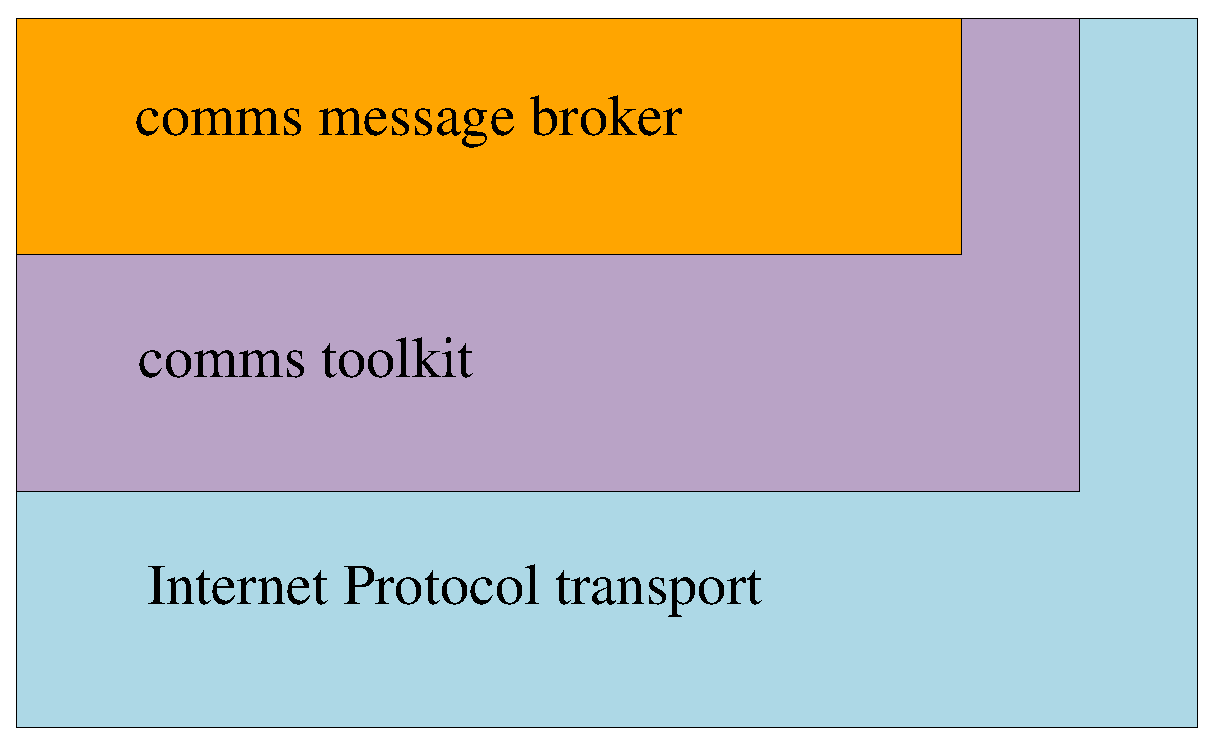
\includegraphics[scale=0.30]{../fig/comms.eps}
\caption{Comms Framework Layers}
\label{FigCommsLayers}
\end{minipage}
\hspace{0.5cm}
\begin{minipage}[b]{0.45\linewidth}
\centering
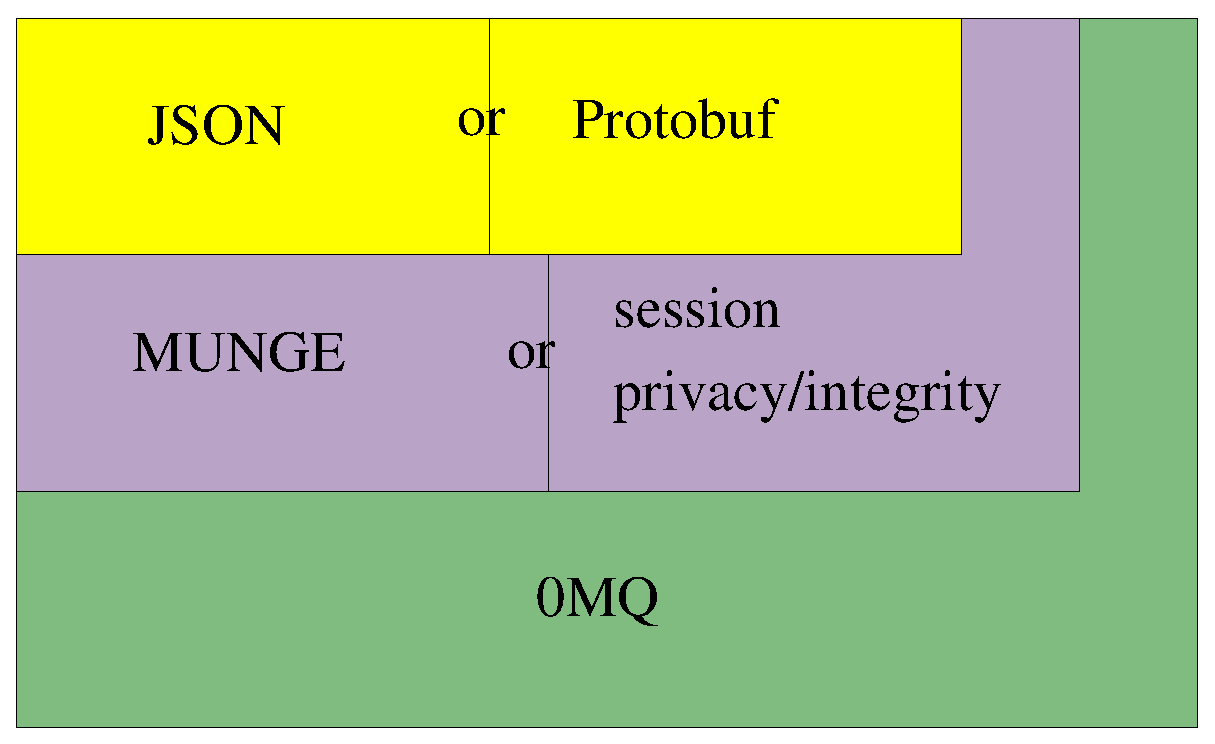
\includegraphics[scale=0.30]{../fig/commstk.eps}
\caption{Comms Toolkit Layers}
\label{FigCommsTK}
\end{minipage}
\end{figure}

\subsubsection{Internet Protocol Transport}

The \ngrm\ comms framework is layered upon IP, and presumes
complete IP level unicast and multicast connectivity, so that any
collection of nodes can be wired up in a comms session without
the need to re-implement the equivalent of IP routing within
the framework.\footnote{Building a reliable 100K node IP internetwork
is a solved problem.} 
The addressing, routing, and subnetting of this IP network is beyond of
scope of \ngrm, except that its design should introduce no single
points of failure (\ref{ReqsHiLevFun}, req. 1.2), should be protected
from external intrusion, and should avoid performance bottlenecks which
would unnecessarily constrain the resource manager's node selection options.

The comms framework should support communication over multiple
(fully-routed) network planes, for example using either a management
ethernet or IP-over-IB or both according to the performance/reliability
requirements of the particular application.

Dynamic unicast IP address allocation must be available to support
dynamically created virtual nodes (Linux containers launched with
virtual network interfaces).  Similarly,
dynamic multicast address allocation must be available to support
private multicast groups within dynamically created comms sessions.
These requirements can be addressed by existing technology such as
DHCP\cite{rfc2131} and MADCAP\cite{rfc2730}.

A private DNS\cite{rfc1034} is used by the comms framework to
map a hierarchical namespace to the comms session hierarchy.
The root comms session has the root domain name, e.g. ``{\tt \ngrm.}'',
and the root server contains address records for all hosts in the domain, e.g.
``{\tt n1.\ngrm}'', ``{\tt n2.\ngrm}'',..., ``{\tt n99999.\ngrm}''.
Comms sessions spawned by the root session get their own sub-domain, e.g.
``{\tt s1.\ngrm}'', ``{\tt s2.\ngrm}'', ``{\tt s3.\ngrm}'',
and contain address records for the nodes assigned to them, e.g.
``{\tt n1.s1.\ngrm}'', ``{\tt n2.s1.\ngrm}'', ``{\tt n3.s1.\ngrm}''.
Sub-domains are created for each level of comms session recursion.
Each session runs a set of DNS servers for its domain.
When a node joins a new session, its DNS resolver is reconfigured to use
the session DNS servers and to search the session's DNS domain first,
thus each level of session overlays a new set of names over
the root session's that provides job-centric naming uniformity.
DNS SRV records\cite{rfc2782} provide a rudimentary service location
brokerage within the session.
Well understood techniques for DNS fault tolerance,
caching, and dynamic reconfiguration are leveraged to scale performance
in large sessions such as the root session.

A comms session could optionally be spawned inside a virtual private
network (\ref{ReqsUseCases}, UC21) such that IP communication
is limited to within the comms session.  IPsec\cite{rfc2401} with
a pre-shared session key could be used to provide session integrity and
privacy at the IP layer if desired.

\subsubsection{Comms Toolkit}

The framework provides a toolkit for sending and receiving
protocol messages privately and securely within a session,
with the goals of providing a robust foundation for \ngrm\ components
and promoting rapid development, code reuse, and interoperability.
The toolkit includes messaging libraries,
protocol encoding/decoding libraries, and security options.
Toolkit pieces can be mixed and matched according to application
requirements.  We may cull the comms toolkit as we learn more
about the pieces while prototyping other \ngrm\ components.

Two messaging approaches of interest are \zMQ\cite{ZMQGuide} and
SCTP\cite{SCTP}.
\zMQ\ provides the ability to manipulate opaque, multipart messages,
and carry them across various transports, including TCP and
PGM\cite{rfc3208} (reliable multicast), using a socket-like API.
\zMQ\ sockets can exchange messages using patterns including
REQ-REP (RPC), PUB-SUB, and PUSH-PULL (message stream).
\zMQ\ can be used to build applications or custom message brokers.
Complex message routing topologies such as tree-based overlay networks
(Figure~\ref{FigZmqTBON}) can be built from simple components.
\zMQ\ has a large number of language bindings.

SCTP is an IETF-standardized, message-oriented transport developed
in the telephony world with an implementation in the Linux kernel.
It offers multi-streaming, the bundling of {\em streams} in one
{\em association} (connection).  Individual streams can be configured for
different ordering and reliability semantics.  SCTP supports
multi-homing for reliability and congestion avoidance, and
can transparently generate and check an HMAC for messages using a
pre-shared key to implement message integrity.  Unlike \zMQ, SCTP is
connection-based and does not implement a standardized reliable multicast
mode.

\begin{figure}
\centering
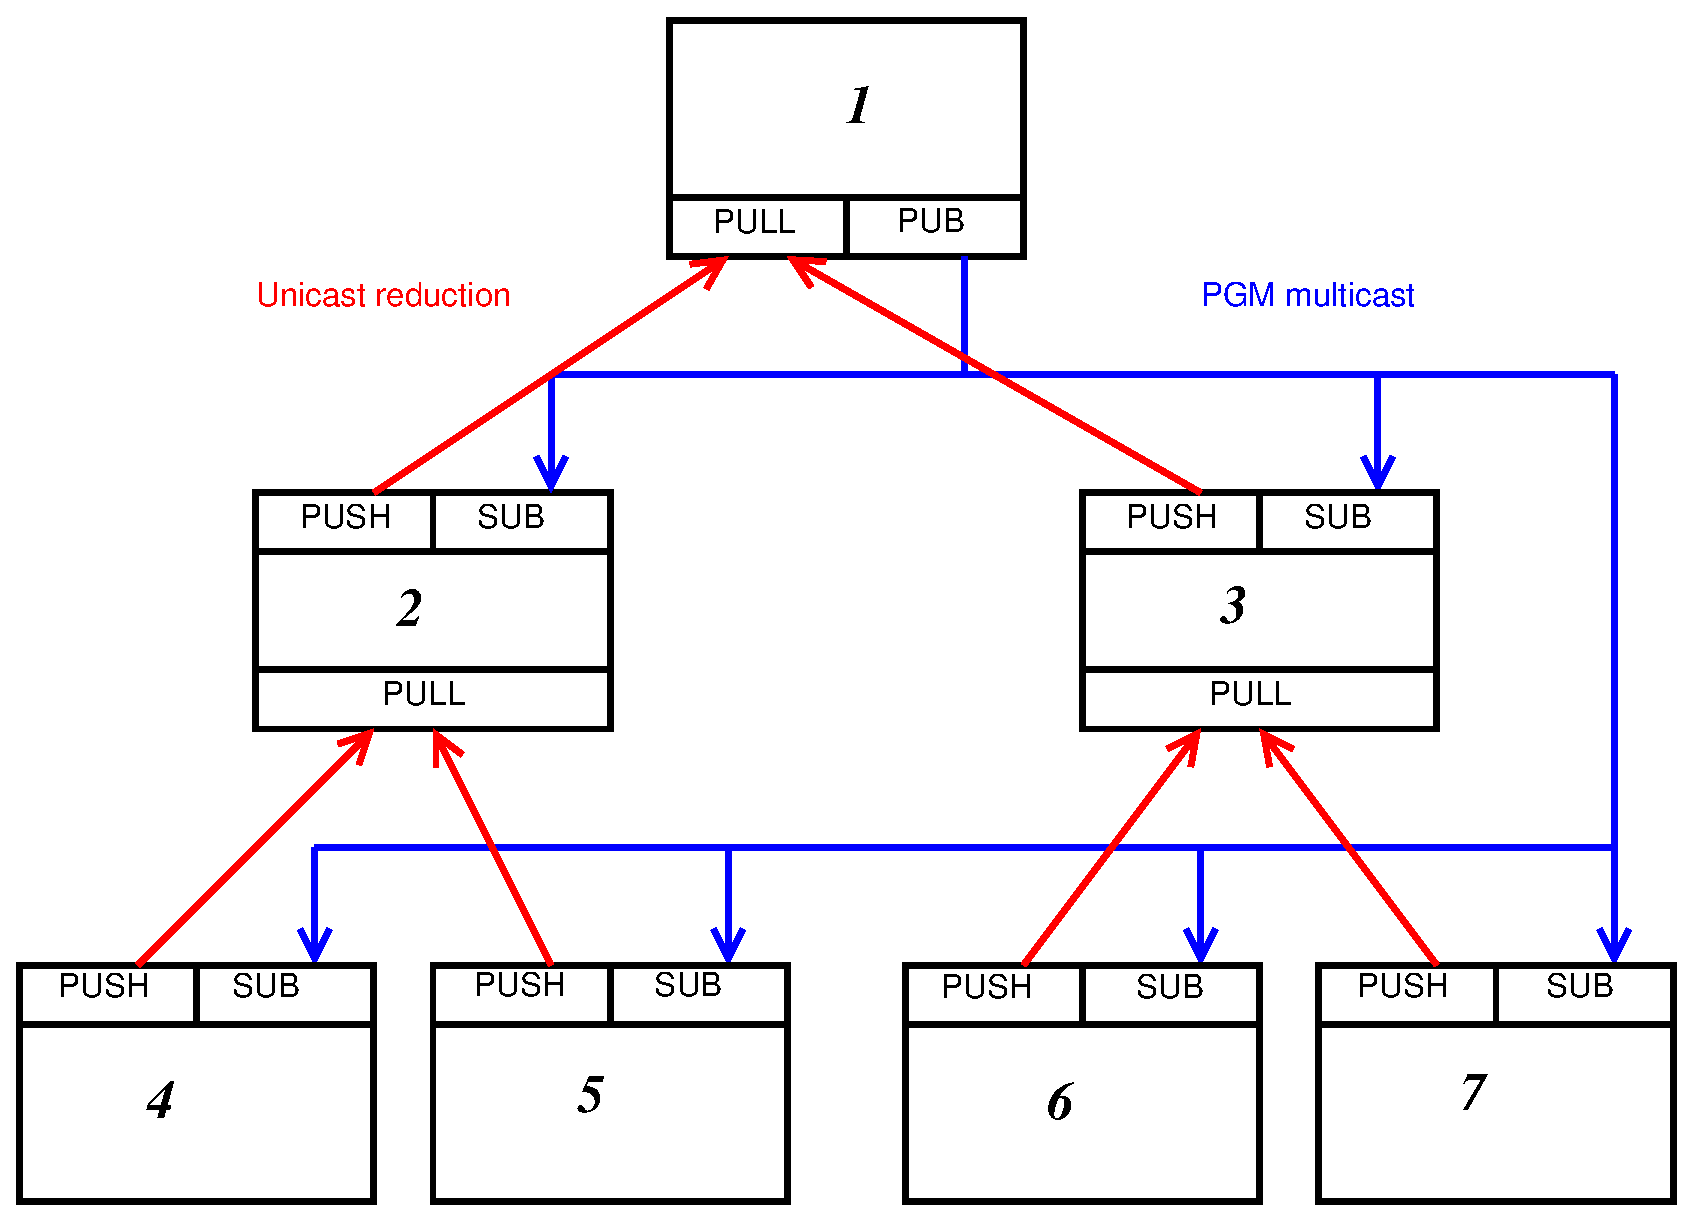
\includegraphics[scale=0.35]{../fig/zmqtbon.eps}
\caption{Tree Based Overlay Network Over \zMQ}
\label{FigZmqTBON}
\end{figure}

Two widely used methods of encoding data in messages are
JSON\cite{rfc4627} 
and Protocol Buffers\cite{Protobuf}.
JSON is a self-describing format
that supports protocol evolution without recompiling endpoints.  It has
many language bindings but it is also space-inefficient and slow.
Protocol Buffers is a compiled format that supports
only limited protocol evolution without recompilation.  It has relatively
fewer language bindings than JSON but is space-efficient and fast.
Depending on the application either may be appropriate.

Message integrity and privacy can be obtained using either a session
security context or via MUNGE\cite{MUNGE}.
Each comms session is allocated a {\em session key} by its parent\footnote{
The root comms session obtains its session key out of band.}
which is used for establishing a shared security context
for messages exchanged within the comms session.
The shared security context allows communicating entities to have integrity
and privacy (from children, siblings, and their children)
without the overhead
of a key exchange for each pair of communicating endpoints.
This is especially useful for non point-to-point comms patterns such as PUB-SUB.
The parent retains state about its offspring including their session keys.
Children forget their parent's key;  thus as comms sessions recurse,
parents get privacy from children but not the reverse.
An application acting as a gateway between parent and child would use
the child's session key as it is known by both parent and child.

If the sender of a message needs to be authenticated, or if messages must
be kept private from other users within the session or its anscestors,
messages can be enclosed as payload in a MUNGE\cite{MUNGE}
credential.
In order for this to work, \ngrm's comms framework must operate within a
single MUNGE security realm,
which implies a single single administrative domain with consistent
user and group identities.

\subsubsection{Comms Message Broker}\label{SecCommsCMB}

Within a comms session, a distributed comms message broker (CMB)
is established to provide basic session services.
The CMB is responsible for launching new sessions,
managing session membership,
detecting and adapting to session node failures,
providing a basic event messaging system,
and starting other \ngrm\ components.

\paragraph{Architecture}
The CMB is a distributed service with nodes interconnected in a topology
that is to be determined.
A distinguished {\em control node} serves as the heart of the CMB.
The control node is distinguished because it alone communicates with
the parent session, and it holds the master copy of the session state.
For fault tolerance, there is a primary and backup control node for each
each session, with the parent CMB initiating any takeover.
Interfaces exposed by the control node to the parent are always passive;
that is, the parent initiates connections and makes requests or subscribes
to events, and the child control node responds or publishes events.

\paragraph{Session State}
The CMB implements a simple key-value store to manage the
internal state enumerated in Table~\ref{TabCMBState}.
The session state for the largest session is small enough to easily
fit in memory.
The master state lives on the control node.
Slave caches on other nodes are loosely consistent with the master copy:
reads may utilize a local or peer cache;
writes are through to the control node.
Each write on the control node updates the key's generation number,
its value, and triggers a state update event which
can be used to update caches and synchronize other software using the
state.

\begin{table}
  \centering
  \begin{tabular}{| l | p{0.6\textwidth} |}\hline
  \textbf{Name} & \textbf{Description} \\
  \hline
  cmb.cred = $key$ &
        My session key.\\
  cmb.fqdn = $name$ &
        Fully qualified domain name for the session.\\
  cmb.nodeset = $nodelist$ &
        List of my nodes.\\
  cmb.addrs.$node$ = $addrs$ &
        List of addresses for $node$, for forming DNS address records.\\
  cmb.topology.up.$node$ = $nodelist$ & 
        Upward peers for $node$ in CMB topology.\\
  cmb.topology.dn.$node$ = $nodelist$ &
        Downward peers for $node$ in CMB topology.\\
  cmb.alive.$node$ = $yes|no$ &
        Liveness for $node$.\\
  cmb.alloc.$node$ = $yes|no$ &
        Allocation status for $node$.\\
  cmb.attrs.$node$ = $attrlist$ &
	Role attributes assigned to $node$, e.g. ``dns'' and ``control''.\\
  cmb.subscribe.$key$ = $nodelist$ &
        List of nodes subscribed to $key$.\\
  cmb.exec = $cmdline$ &
        Executable to bootstrap on each node.\\
  \hline
  cmb.child.sessions = $sessions$ &
        List of active child sessions.\\
  cmb.child.$session$.cred = $key$ &
        Child sesion key.\\
  cmb.child.$session$.control = $nodelist$ &
        Control node(s) for $session$.\\
  cmb.child.$session$.dns = $nodelist$ &
        DNS server nodes for $session$, for forming DNS NS records.\\
  \hline
  \end{tabular}
  \caption{Comms Message Broker State}
  \label{TabCMBState}
\end{table}

\paragraph{Event Messaging}
The CMB implements a session-wide event messaging service.
Clients of the CMB on any node can publish a $(key, message)$ event tuple.
Other clients can subscribe to events by key.  The CMB ensures that
event messages are routed internally from publishers to subscribers.
The event service is reliable, and for events originating on the same node,
sequenced for in-order delivery.
Events are not queued for late subscribers.
There is a special {\tt event.sched.trigger} event sent out periodically
to synchronize the CMB's internal functions (and those of any other
subscribers to the event) across the session with the goal of minimizing
disruption to bulk-synchronous workloads running within the session.

\paragraph{Session Membership}
The CMB maintains the current {\em nodeset} as part of the session state.
The CMB arranges for the nodeset to be mirrored in private DNS servers
serving up the session's subdomain.
The nodeset may grow or shrink in response to higher level software
allocating/freeing nodes from the parent, or creating/destroying 
virtual nodes within the session.
Nodeset updates will be accompanied by internal topology updates, provided by
the software making the nodeset change or by the CMB itself depending
on the situation.
State update events will be published for the nodeset and topology changes.
While nodes are allocated to a session, they remain in the parent nodeset,
tagged as {\em allocated}.  They forget the parent's session state and key.
When nodes are freed back to the parent, the parent CMB, having subscribed
to the child's nodeset update events, contacts the freed node (using the
child session key) and brings it back online in the parent sesssion.  

\paragraph{Liveness Monitoring}
The CMB maintains the {\em liveness} of its nodes as part
of the session state.
Liveness is assessed by forcing member nodes to communicate with the CMB
at minimum intervals, synchronized by the aforementioned trigger event.
If the CMB has not heard from a node for some number
of trigger periods, it is marked down.
If it finally is heard from, it is marked {\em up}.
In some cases the CMB control node may adjust its internal topology
to account for such changes.
As described above, session state changes trigger state change events.
Higher level software wishing to react to node liveness changes can
subscribe to state change events.
The parent continues to track liveness of nodes allocated to a child by
subscribing to liveness updates via the child's control node.  A trivial
utility that asks the CMB for a list of down nodes in the current session
can be written that works equally well at any level of recursion,
even at the level of the root session.

\paragraph{Node Bootstrap}
A cold started node (or restarted CMB daemon) joins the root session,
obtaining the root session key and the identity of a peer to copy the
session state from out of band in a secure manner.
If the CMB is cold starting after crashing while assigned to
a session other than the root, the CMB of the root and subsequent owning
sessions re-add the node from child to child until there are no children
left or it is evicted according to the policy of an owning session.

\paragraph{Executable Bootstrap}
In order to bootstrap other \ngrm\ components, the CMB daemon, upon
joining a new session, launches a single process on each node,
determined by the {\tt cmb.exec} state variable.
This process is terminated when the node alters its session membership
to join a child session or return to a parent session.
If the process terminates early, an event is generated.

%\begin{figure}
%\centering
%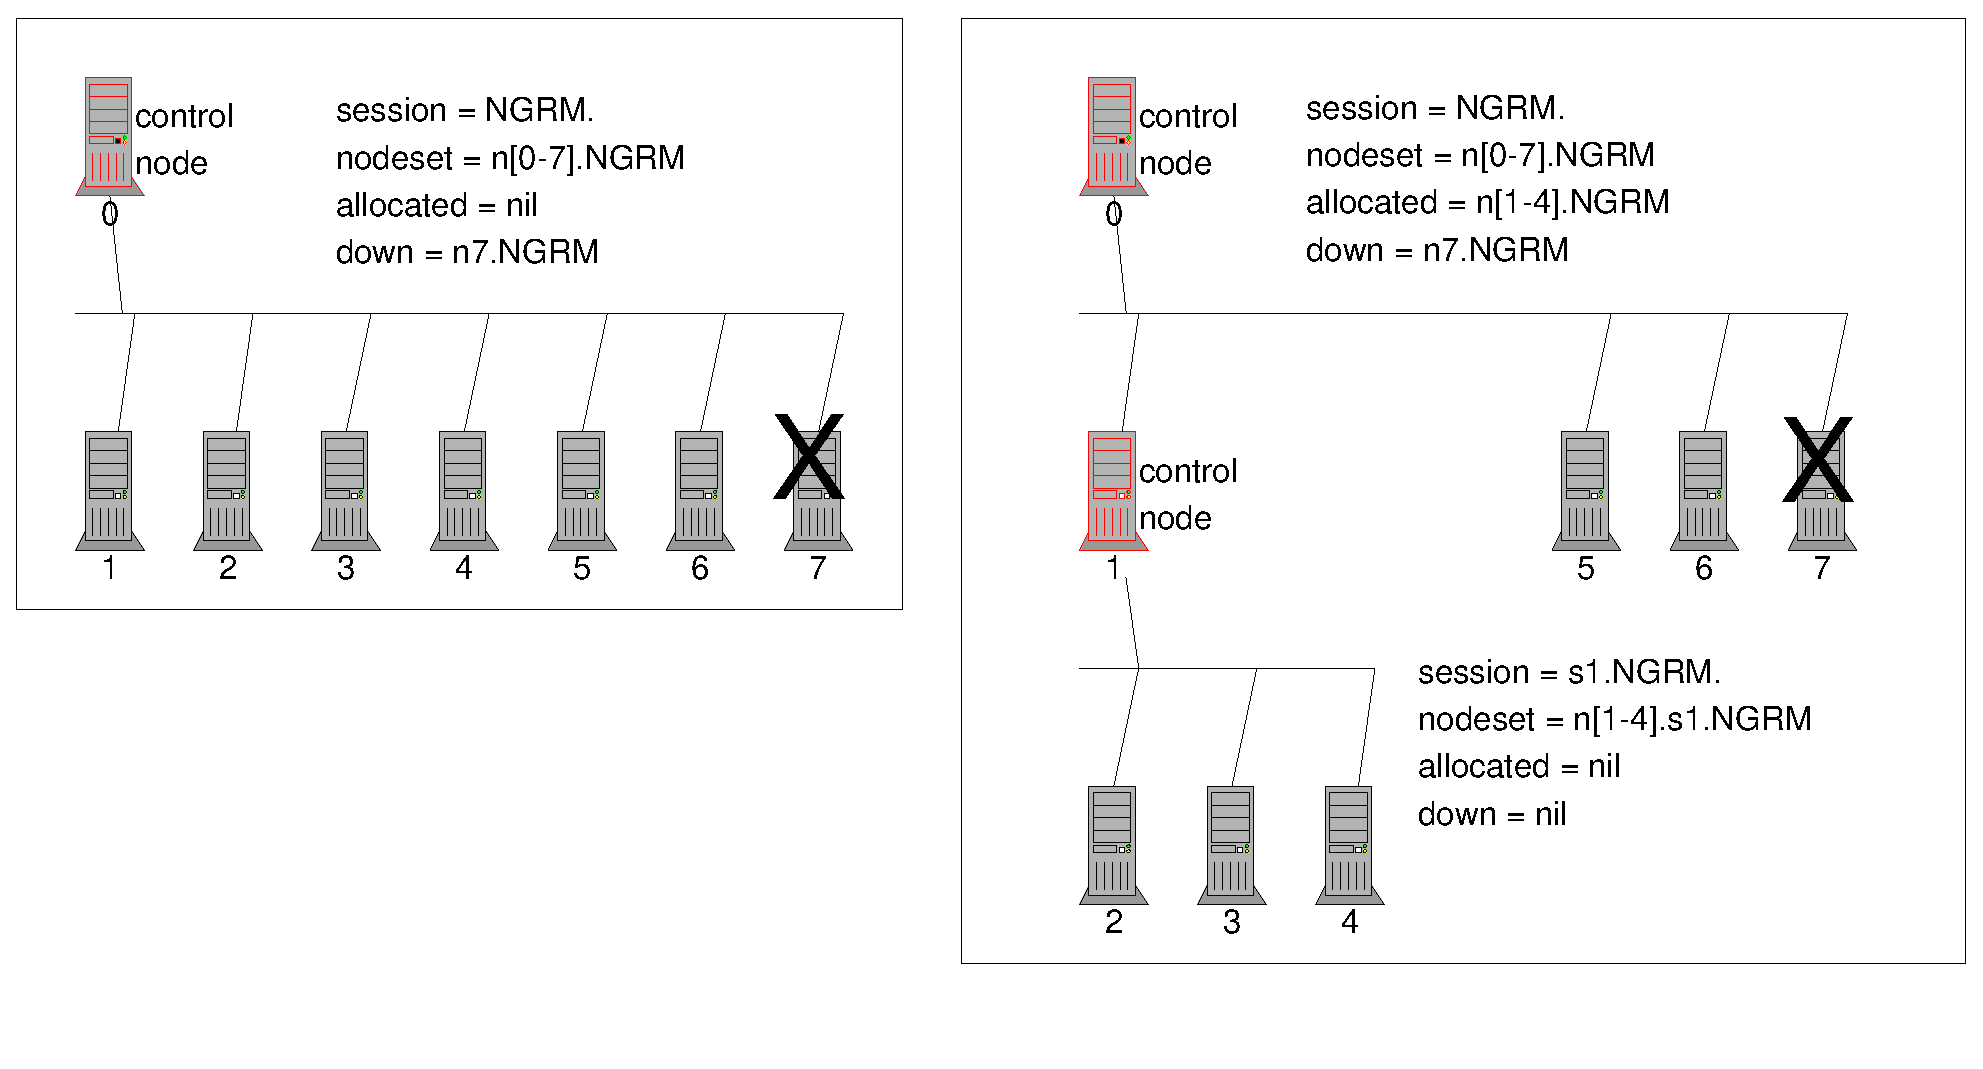
\includegraphics[scale=0.50]{../fig/cmb.eps}
%\caption{Comms Message Broker Spawning a New Comms Session}
%\label{FigCMBSpawn}
%\end{figure}

\paragraph{Session Creation}
The CMB is responsible for the creation of
child comms sessions.
%as shown in Figure~\ref{FigCMBSpawn}.
A child session is created by building the child session state,
updating the current (parent) session state, then sending the
child control node(s) the full session state, and the rest of the nodes
just the new session key and sufficient information to wire up to their
peers in the internal toplogy.
The DNS is updated in the parent to delegate authority
for the new subdomain to the child's DNS servers.
DNS servers are bootstrapped in the child, and the resolver is updated
on member nodes to reflect the new session.

\paragraph{Session Destruction}
The CMB destroys a child comms session by sending a message to the child's
control node requesting that a shutdown event be sent out session wide.
As nodes leave the child nodeset, the parent reclaims them as described 
above in the Session Membership paragraph.
If something goes wrong, the parent can short-circuit the ``clean shutdown''
and actively reclaim nodes as above, as though they had already left the
child nodeset.
The DNS is updated in the parent to remove references to the session's
subdomain.

\subsubsection{Aggregation/Reduction Network}

The \ngrm\ runtime and monitoring components will require an
aggregation/reduction framework similar to MRNet\cite{MRNet} that
can aggregate or reduce data produced across the session before it is
consumed at the control node.

This overlay network should utilize CMB services to respond to support changes
in comms session membership (elasticity).

FIXME: Pull in Dong's requirements/description.
Why not use MRNet?
Can this be part of CMB?

\subsection{Plugin Framework}

TBD

\subsection{Software Development Practices}

TBD

\newpage
\subsection{Framework WBS}\label{FrameworkWBS}

\begin{longtable}{|p{1cm}|p{10.2cm}|p{1cm}|p{1cm}|p{1.8cm}|}\hline
  \textbf{Item} & \textbf{Description}
		& \textbf{Deliv}\footnote{SD = software drop,
			DR = design review, V = viewgraphs, D = document}
		& \textbf{Weeks} & \textbf{Depend} \\
  \hline
  \hline
  \multicolumn{5}{|l|}{1.1. \textbf{Communications Framework}} \\
  \hline
  1.1.1.  & \zMQ\ evaluation.
          Consider CMB and aggregation/reduction design based on \zMQ.
          How does PGM implement reliable message delivery?
          Is the connectionless model a serious problem? 
          Is the implementation robust?
          How would security be integrated?
	& V
	& 2
	& \\
  \hline
  1.1.2.  & SCTP evaluation.
          Consider CMB and aggregation/reduction framework design based on SCTP.
          Compare performance with \zMQ.
          Is the Linux SCTP implementation robust?
          How would security model be integrated?
	& V
	& 4
	& \\
  \hline
  1.1.3.  & MUNGE key change capability to make large MUNGE realm manageable.
	  Add support for multiple keys with lifetimes per bug \#XXXX.
	& SD
	& 
	& \\
  \hline
  1.1.4.  & Design fully routed management and IB networks for all
          Linux clusters in the Livermore Computing collaboration zone.
          Evaluate DNS, DHCP, and MADCAP (or alternative) software
	  and develop deployment strategy.
          Design should be reviewed by LC networking and security staff
	  and published as model for similar efforts.
	& V
	& 
	& \\
  \hline
  1.1.5.  & Investigate IPsec scalability for a comms session.
          Can Linux IPsec implementation handle 100K security association
	  (SA) table entries?
	& V
	&
	& \\
  \hline
  1.1.6.  & CMB I design/prototype.  Develop CMB API's and a protoype
          implementation with a centralized architecture that scales
          to approx 256 nodes.   Stablize API's and allow dependent
	  development to proceed.  Replace "whatsup" Cerebro tool on hype.
	& DR, SD, V
	&  
	& 1.1.1, 1.1.2, 1.1.5 \\
  \hline
  1.1.7.  & Document CMB API's and comms toolkit usage for \ngrm\ components.
          Develop toy application(s) demonstrating usage.
	& V, D
	&  
	& 1.1.1, 1.1.2, 1.1.5, 1.1.6 \\
  \hline
  1.1.8.  & CMB II design/prototype.  Design/prototype CMB II 
          implementation with a distributed architecture that scales
          to 100K nodes.   No fault tolerance.  Replace "skummee"
          in-band data collection on hype and whatsup in LC production.
	& DR, SD, V
	&  
	& 1.1.6, 1.1.3, 1.1.4, 1.1.7 \\
  \hline
  1.1.9.  & CMB III design/develop.  Final implementation with full
	  scalability and fault tolerance.
	& DR, SD, V
	&  
	& 1.1.8 \\
  \hline
  1.1.10. & aggregation/reduction framework design/prototype.
	& DR
	&
	& 1.1.7\\
  \hline
  1.1.11. & Implement aggregation/reduction framework.
	& SD
	&
	& 1.1.10\\
  \hline
  \multicolumn{5}{|l|}{1.2. \textbf{Plugin Framework}} \\
  \hline
  1.2.1   & Design/prototype plugin framework
	& V, D
	& 
	& \\
  \hline
  \multicolumn{5}{|l|}{1.3. \textbf{Software Development Practices}} \\
  \hline
  1.3.1   & Codify project software development practices.
	& V, D
	& 
	& \\
  \hline
\end{longtable}


\section{Resource Management Thrust}


\section{File System Provisioning and System Monitoring}

This section describes the file system provisioning and system monitoring
subsystems of \ngrm.  By coupling these systems to the resource manager,
we achieve our goals of mitigating system noise, improving job launch time,
and promoting reproduceability and data provenance.

\subsection{File System Provisioning}

We use the term "file system provisioning" to describe how executables
and other read-only data are provided to compute nodes.
A provisioning system based on immutable datasets is proposed.
Immutable datasets are collections of files that can be aggressively cached
without revalidation,
and reliably referenced in a job record for data provenance.
In the proposed system, a dataset is stored in a container,
actually itself a file formatted as a local file system such as ext4 or
squashfs.  The container, which is stored in a special dataset repository,
is exported as a read-only network block device,
then mounted like a regular local file system on compute nodes,
where the files that comprise the dataset are individually accessible.
The system can be used to provision the root file system,
or any other file system provided its content can be stored immutably
in a dataset container and managed in the dataset repository.

The provisioning system consists of the
distributed network block device,
dataset repository,
tools for creating and managing datasets,
and the resource manager interfaces for assigning datasets to jobs
such that they become part of a job's runtime environment and
are referenced in the job's historical record.


\subsubsection{Distributed Network Block Device}

A network block device driver based on 9P protocol called 9nbd\cite{9nbd}
was prototyped in August 2012.
9nbd, which at a high level has functionality similar to iSCSI or SRP,
leverages the existing kernel 9P transport to access a backing file
in a remote 9P file system.
A hierarcically distributed, shared network block device can be built
using 9nbd and any number of levels of chained 9P diod\cite{diod}
I/O forwarding servers, fanned out in a hierarchy as depicted in
Figure~\ref{Fig9nbd}.
\begin{figure}
\centering
\fbox{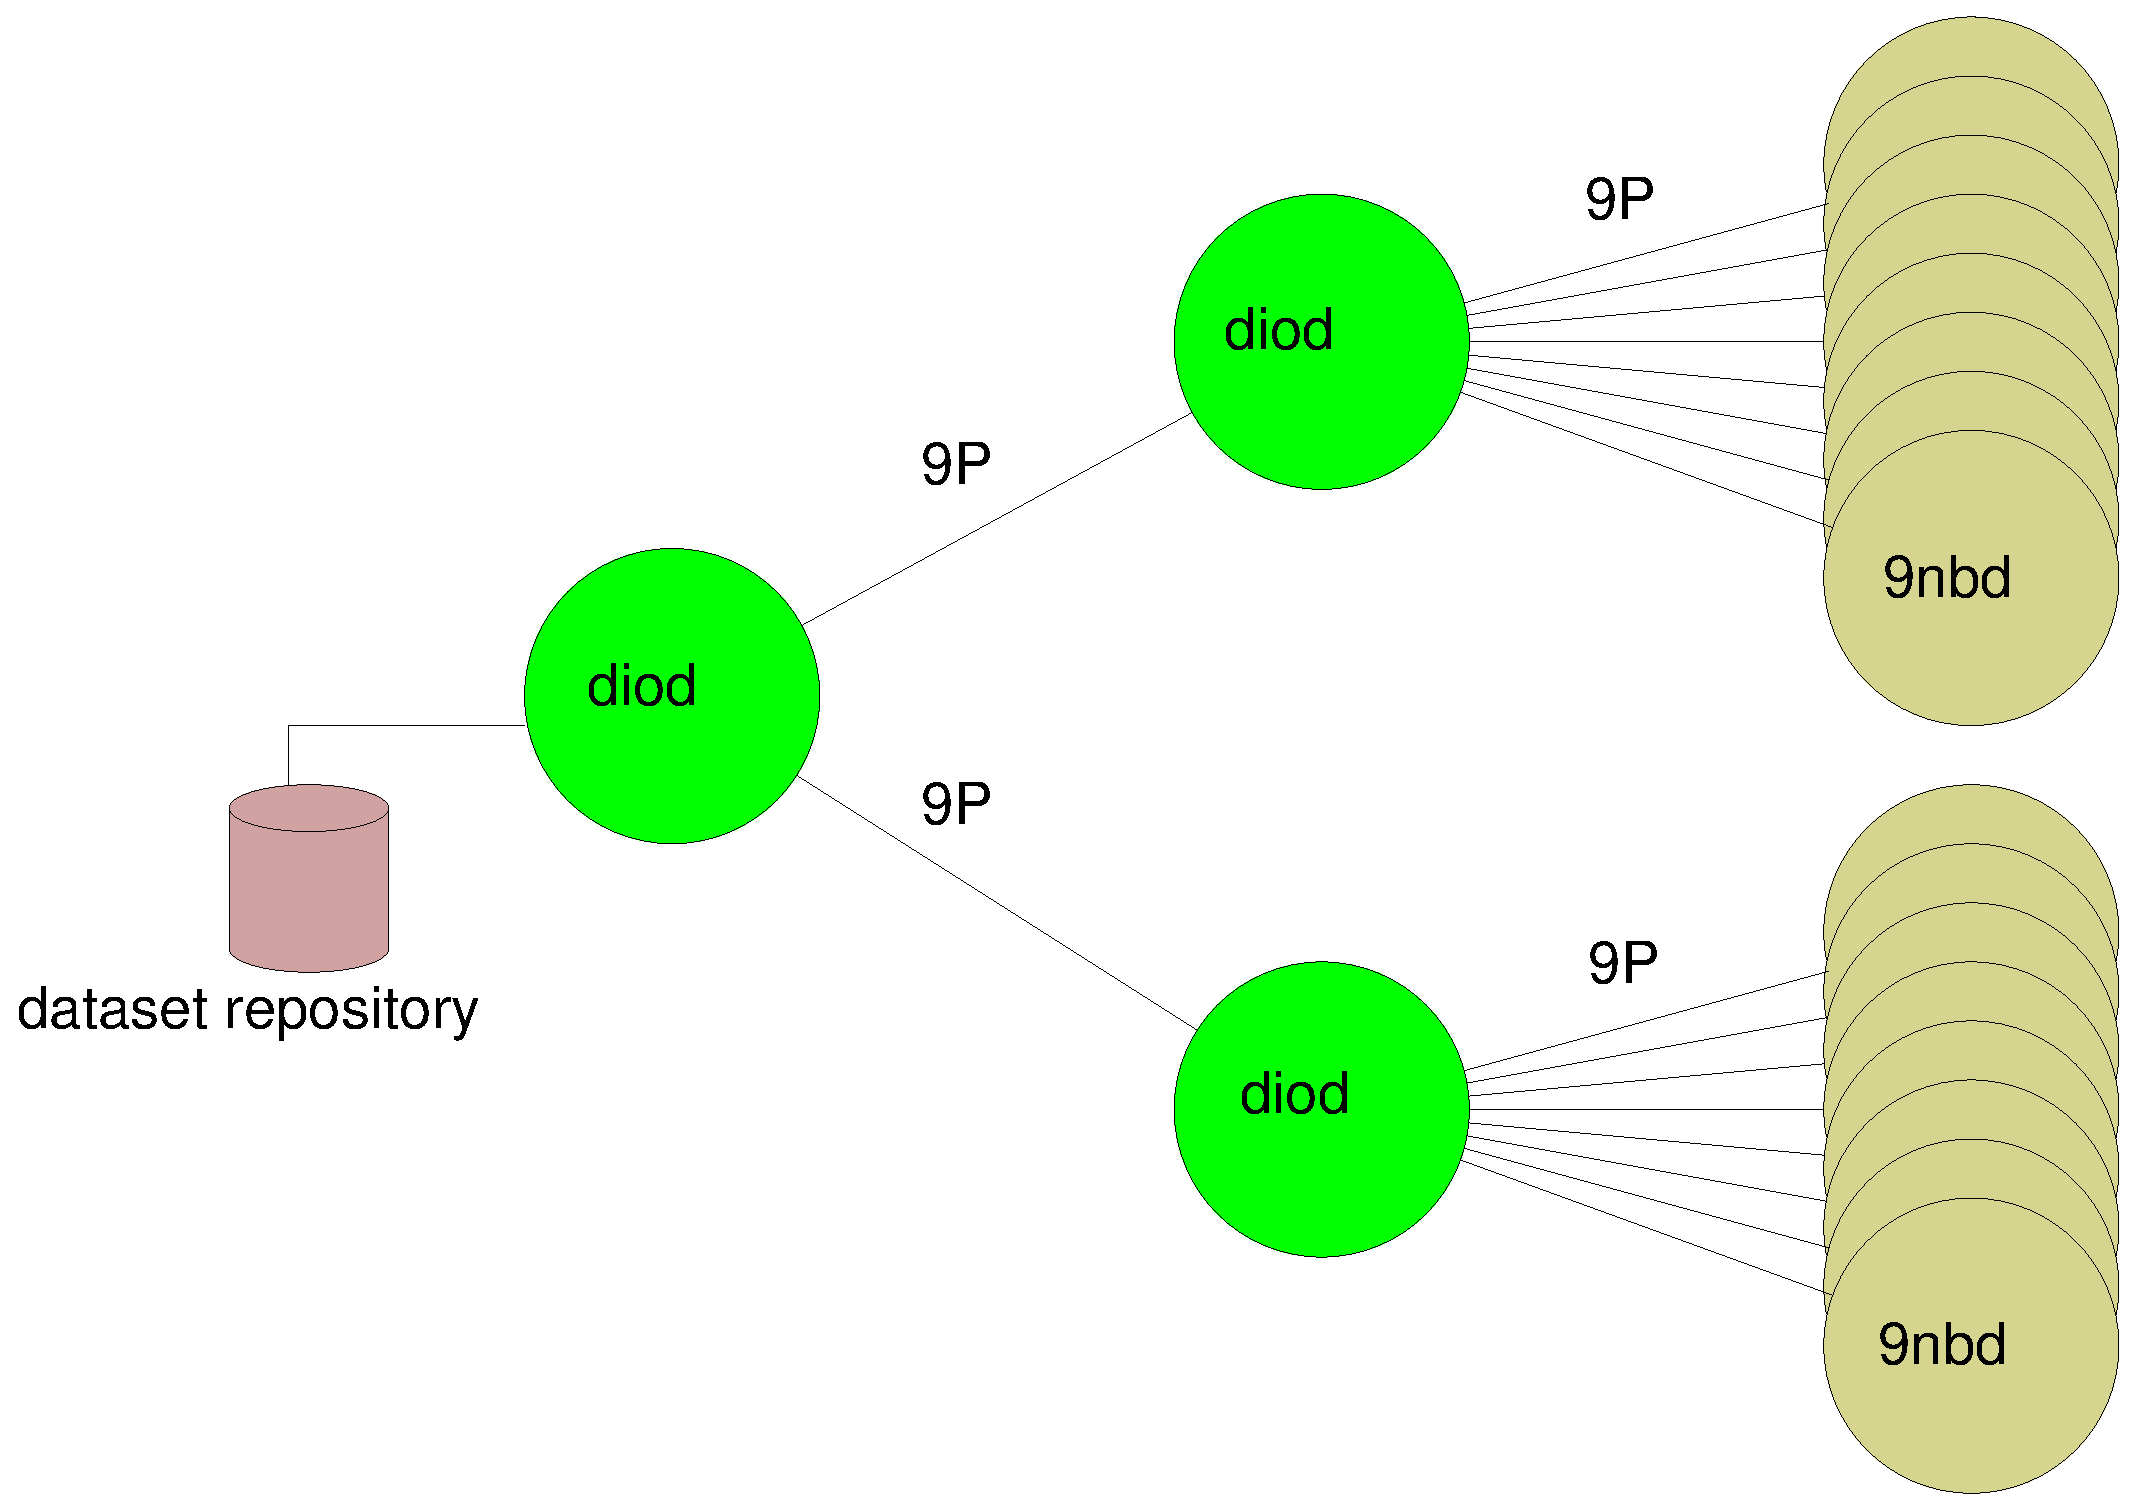
\includegraphics[scale=0.30]{../fig/dnbd.eps}}
\caption{
Immutable, read-only datasets residing in repository are forwarded by diod
I/O forwarding server to compute nodes running 9nbd where they appear
as block devices.  Block devices are mounted on compute nodes with
the semantics of a local file system.
}
\label{Fig9nbd}
\end{figure}

\paragraph{Performance Outlook}
A diod I/O forwarding server will read the working set of the container
file in once and thereafter serve it from its page cache to multiple clients.
At each compute node,
the block device driver naturally caches its working set in the buffer cache,
which is optimized for many common file system usage patterns,
such as path search and dynamic library loading.
A study of parallel path search\cite{BlkDevPathSearch}
using ext4, the {\em loopback} block device, one level of diod I/O forwarding
with a fanout of 82 to 1, and a single NFS server,
showed flat scaling to 82 nodes, the largest scale attempted,
while NFS began to slow at eight nodes.
This result, depicted in Figure~\ref{FigPathWalk},
indicates that the distributed block device based on 9P has
great promise to improve job launch times over NFS, and the flexible
hierarchical architecture should easily scale to 100K nodes, although
testing with more than one level of diod forwarding may identify some
additional work required to get there.
\begin{figure}
\centering
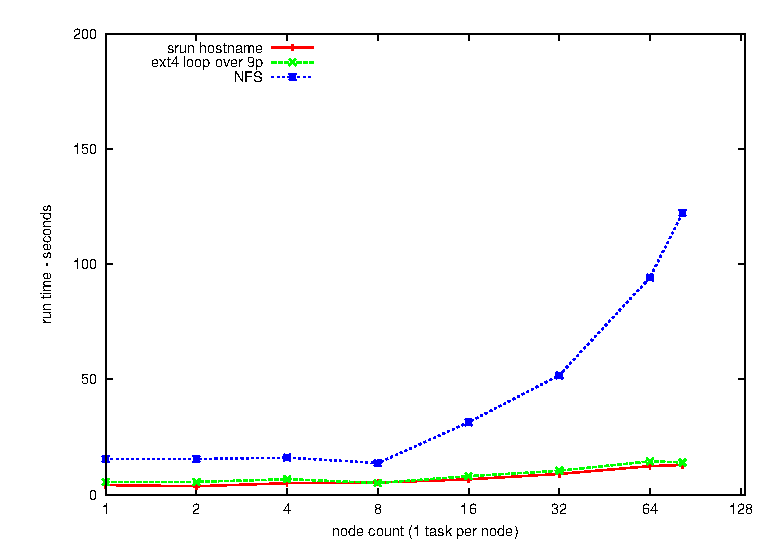
\includegraphics[scale=1]{../fig/pathwalk.eps}
\caption{
Path walk performance for distributed block device based on 9P and diod
scales the same as the null slurm job up to 82 nodes, while NFS begins
to slow at 8 nodes.
}
\label{FigPathWalk}
\end{figure}

\paragraph{System Noise Outlook}
The distributed block device requires no cache management as the
data is read-only throughout the system.  Unlike NFS (even mounted read-only),
compute nodes will not attempt to asynchronously revalidate cached
attributes or data, since the entire dataset is immutable.
Data in the buffer cache is never dirty, and can be thrown out and at
any point should the application require the memory, and reread on demand later.
Therefore, the approach is very friendly to applications running on compute
nodes, with a system noise footprint that can be near zero.

\paragraph{Security}
The 9nbd prototype and diod server implement MUNGE authentication
over the built-in TCP transport plugin, and no integrity or privacy.
The \ngrm\ comms framework security model should be leveraged,
by adding an \ngrm-specific kernel 9P transport plugin,
to obtain integrity and privacy for I/O forwarding within a comms session,

\paragraph{Resiliency}
The 9nbd prototype implements single server resiliency, where the
9nbd block device driver can re-establish the transport and replay
9P connection state to a new server instance should the server reboot.
The client blocks while this recovery takes place.
The \ngrm\ comms framework CMB should be leveraged,
by adding an \ngrm-specific kernel 9P transport plugin,
to obtain multi-server resiliency based on storing possible diod server
identities in the CMB state and tracking liveness changes.
The client can thus recover more quickly by leveraging the CMB.

\paragraph{Root File System Special Needs}
Provisioning the system root file system to diskless nodes requires
some additional care and is somewhat distribution specific.
Root has to be mounted from a limited initramfs environment, which
implies that MUNGE and 9nbd have to be functional in that environment.
For distributions based on Red Hat Enterprise Linux, a {\em dracut}
module is needed for both MUNGE and 9nbd.  Once root is mounted, it can
remain read-only, or more conveniently, it can be combined with a {\em zram}
memory-based block device using {\em dm-snapshot}, making it appear
writable, with any changes going to RAM.  The dracut modules and the
dm-snapshot/zram support can be added to the nfsroot\cite{nfsroot}
software package.

\subsubsection{Dataset Repository}

Dataset containers can initially be stored in NFS, Lustre, or a local file
system and managed by system administrators using simple scripts.
However, there are a few practical problems with this.
One is that a large number of nearly identical containers may proliferate
and use too much space.  Another is that there is no mechanism to enforce
the immutability of a dataset under a given file name, and no way
to incorporate job record references (e.g. a use count) into a repository
purge policy.
Finally, the intent is to allow users to manage the content of their datasets,
but user access must be controlled such that containers are always
valid file system images and container metadata is properly filled in.
These three factors motivate the need for a specialized dataset repository.

\paragraph{Copy-on-write}
A large number of nearly identical containers may proliferate, for example
if a dataset is undergoing iterative changes during development.
Ideally the file system storing dataset containers will support
{\em thin copies} or block level {\em de-duplication} so that only one
copy of unchanged content is stored.

\paragraph{Content Addressable}
To prevent datasets from changing while mounted, which would trigger
kernel panics, and from run to run, which would affect provenance and
reproduceability, the file system storing dataset containers should
be content addressable.  For example, instead of a file name, a cryptographic
hash of its content is used to refer to a container file.
The file system or the repository interface should enforce this atomically.

\paragraph{Container Format and Repository Model}
Containers must contain valid file system images in order to avoid
mount errors or kernel panics, and certain metadata should be associated
with containers to record information about how it was created.
The resource manager will take references on containers when they are used
and when they are referenced by a job's provenance record.
Thus the dataset repository is more than a file system that has
content addressability and copy-on-write.
It must enforce provisioning system policy over container additions and
removals and ensure that all its containers have a valid format.

\subsubsection{Tools for Creating and Managing Datasets}

Tools similar to those provided for package management are required to
create valid containers with proper metadata from collections of files,
for managing and updating containers, and for interacting with the repository.
Stakeholders such as system administrators and code teams who might
be interested in creating datasets should be consulted to understand
their workflow and tool needs.  

\subsubsection{Resource Manager Interface}

The provisioning system is intended to be used in conjunction with
the \ngrm\ runtime's capability of configuring the file system
namespace (e.g. set of mount points) on a custom basis for each job. 

FIXME: launching a custom I/O forwarding topology within the job
vs fixed topology.

FIXME: taking a reference on a container while it is mounted and
from job log for provenance.

\subsubsection{File System Provisioning WBS}

\begin{longtable}{|p{1cm}|p{10.2cm}|p{1cm}|p{1cm}|p{1.8cm}|}\hline
  \textbf{Item} & \textbf{Description}
                & \textbf{Deliv}\footnote{SD = software drop,
                        DR = design review, V = viewgraphs, D = document}
                & \textbf{Weeks} & \textbf{Depend} \\
  \hline
  \hline
  \multicolumn{5}{|l|}{3.1. \textbf{Distributed Network Block Device}} \\
  \hline
  3.1.1.& Complete initial 9nbd network block device development, including
          backport upstream 9P transport fixes, refine/test 9nbd resiliency
          code, submit for LKML integration.
        & SD
        & 
        & \\
  \hline
  3.1.2.& (root file system only) Add MUNGE key bootstrap and 9nbd root
	  support to nfsroot dracut module.
        & SD
        & 
        & \\
  \hline
  3.1.3.& (root file system only) Backport zram TRIM support so space
	  can be reclaimed in zram-based root file systems.
        & SD
        & 
        & \\
  \hline
  3.1.4.& Design/develop initial container format and rudimentary scripts
	  for creating containers for manually managed NFS dataset repository.
        & SD
        & 
        & \\
  \hline
  3.1.5.& Production release of distributed network block device
	  with root file system support.
	  Support booting up to 4000 nodes from a container stored
	  on a Netapp NFS filer, and forwarded via one level of diod
	  I/O forwarding.
	  Implement single node resiliency and MUNGE authentication
	  (no privacy or integrity).
        & SD
        & 
        & 3.1.1, 3.1.2, 3.1.3, 3.1.4\\
  \hline
  3.1.6.& Performance study at scale of direct NFS vs distributed block
	    device, including Pynamic, pathwalk, and FTQ.
        & V
        & 
        & 3.1.5 \\
  \hline
  3.1.7.& Explore best way to remount multiple levels of diod servers.
          Use v9fs with cache=loose?  Is more work needed to allow
	  arbitrary levels of I/O forwarding?
        & V
        & 
        & \\
  \hline
  3.1.8.& Design/prototype 9P transport plugin that leverages the \ngrm\ 
	  comms framework for resiliency and privacy/integrity.
        & DR
        & 
        & \\
  \hline
  3.1.9.& Implement 9P transport plugin.
        & SD
        & 
        & 3.1.8\\
  \hline
  \multicolumn{5}{|l|}{3.2. \textbf{Dataset Repository, Tools, and \ngrm\ Integration}} \\
  \hline
  3.2.1.& Design/prototype SLURM SPANK plugin that allows users
          to select among available root images.  Manage private file system
          namespace for user, perform post-mount configuration, perform uid
          mapping.  Develop strategy for handling mounts such as home
          directories that would be overmounted by a new root.
        & DR
        & 
        & 3.1.5 \\
  \hline
  3.2.2.& Design/prototype container format and tools for
	  creating/managing datasets.
	  Consult with stakeholders to understand workflow.
	  Demo prototype and iterate.
        & DR
        & 
        & \\
  \hline
  3.2.3.& Design/prototype dataset repository with copy-on-write/dedup,
	  content addressability, repo contract enforcement.
        & DR
        & 
        & \\
  \hline
  3.2.4.& Implement tools for creating/managing datasets.
        & SD
        & 
        & 3.2.2 \\
  \hline
  3.2.5.& Implement dataset repository.
        & SD
        & 
        & 3.2.3 \\
  \hline
  3.2.6.& Design/prototype \ngrm\ integration including
	  private file system namespace management,
          RM management of dataset references during execution and in job
	  record,
	  RM launch of private diod daemons.
	  (co-design with \ngrm\ runtime?)
        & DR
        & 
        & 3.1.5, 3.2.1, 3.2.3, 3.2.4 \\
  \hline
  3.2.7.& Implement \ngrm\ integration.
        & SD
        & 
        & 3.2.6 \\
  \hline
\end{longtable}
\newpage

\subsection{System Monitoring}

\ngrm\ system monitoring consists of three main components:
a plugin system which allows user and system defined code to execute
periodically to check for anomolous situations or take data samples,
a monitoring console which aggregates the state of resources within a
comms sesssion and presents it in the form of a web page for users and
support staff, and a NoSQL monitoring database used to store data for
offline analysis and data provenance.
These subsystems are layered upon the comms framework event messaging and
aggregation/reduction services.  The general approach is to allow monitoring
to be customized within a session, with the parent session delegating
the responsibility for monitoring to its children.

\subsubsection{Monitoring Plugin System}

The monitoring plugin system provides a facility for arbitrary code to be
periodically executed across a session.  To minimize disruption to
bulk-synchronous workloads, this execution is synchronized by the 
session scheduling trigger event.  The set of active plugins is
under the control of the session owner, with some reasonable
defaults provided that can be overridden.

The details of the plugin structure is a design activity, however,
an example of a possible solution is for plugins to take the form of
Lua scripts loaded into the CMB state database
(thus shared across the session) and executed in the context of
a monitoring daemon with an embedded Lua interpreter.

Plugins have three main functions: data source, data reduction,
and data sink.  The data source function is driven by the scheduling
trigger and may directly publish events, for example if a monitored
value exceeds a threshold, or produce structured data for the
aggregation/reduction network.
The data reduction function aggregates structured data from instances
of the plugin's source function.
For example, a plugin that monitors the total amount of memory used
by the session might register a reduction function that takes the sum of
arriving samples.
Finally, plugins can register a function to sink data at the monitoring
console, rendering it for display, or at points in the session that interface
with the NoSQL monitoring database for persistent storage.

\subsubsection{Monitoring Console}

The monitoring console runs on the session control node and provides
a centralized point for monitoring each session.
An HTTP interface is provided which includes links to the control nodes
of child sessions, thus the entire hierarchy of sessions can be navigated
from the root session with a web browser.
The console displays information about the session that comes directly
from the comms CMB, including its time of inception, node membership,
node liveness, users, and scheduling trigger period.

The set of active plugins and the views created by them are represented.
Events generated by plugins are displayed in a scrollable region.

All the information that is available via the monitoring console web page
is also available via command line tools to a shell user on the session
control node.

\subsubsection{NoSQL Monitoring Database}

The NoSQL monitoring database is a large, centralized, persistent database
that stores structured log data for analysis and data provenance.
Log data is generated by monitoring plugins, but may come from other sources
such as syslog, the \ngrm\ runtime, resource manager, or scheduler.

One reason this database is centralized is to allow queries
to be constructed that correlate failures or performance anomalies
across domains; for example, jobs running slow or producing incorrect
results because of file system problems.  The database will directly
benefit system administrators and suport staff who currently perform
these tasks manually.

By preserving contextual information surrounding the execution of a job,
we enable questions to be asked later on when the same job produces
different results.  This is a central goal of provenance.

The database will need some schema design in order to enable queries
that are operationally useful.  For example, RAS metrics may be obtained
on hardware component failures if we are careful to log enough information
to identify the component (e.g. a double bit memory error at address \#xxxx
versus a failure of dimm with model and serial number).

This effort will leverage the work of an in-progress LDRD
feasbility study\cite{LogLDRD}.

\subsubsection{Monitoring WBS}

\begin{longtable}{|p{1cm}|p{10.2cm}|p{1cm}|p{1cm}|p{1.8cm}|}\hline
  \textbf{Item} & \textbf{Description}
                & \textbf{Deliv}\footnote{SD = software drop,
                        DR = design review, V = viewgraphs, D = document}
                & \textbf{Weeks} & \textbf{Depend} \\
  \hline
  \hline
  \multicolumn{5}{|l|}{3.3. \textbf{Monitoring Plugin System}} \\
  \hline
  3.3.1.& Design/prototype plugin system.
	& DR
	&
	& \\
  \hline
  3.3.2.& Implement plugin system.
        & SD
        &
        & 3.3.1 \\
  \hline
  3.3.3.& Document process for creating monitoring plugins.
        & D
        &
        & 3.3.1 \\
  \hline
  3.3.4.& Design/prototype a set of default plugins including plugins
          for instrumenting jobs to gather "implicit provenance" such as
          file accesses.
        & DR
        & 
        & 3.3.1 \\
  \hline
  3.3.5 & Implement set of default plugins.
        & SD
        &
        & 3.3.4 \\

  \hline
  \multicolumn{5}{|l|}{3.4. \textbf{Monitoring Console}} \\
  \hline

  3.4.1.& Design/prototype monitoring console.
	& DR
	&
	& \\
  \hline
  3.4.2.& Implement monitoring console.
	& SD
	&
	& 3.3.1, 3.4.1 \\
  \hline
  \multicolumn{5}{|l|}{3.5. \textbf{NoSQL Monitoring Database}} \\
  \hline
  3.5.1.& Study available NoSQL databases for 100K node scalability
          and appropriate query interface.
          Use offline log data to investigate system diagnostic capability
          and prototype queries.
          (Gamblin/Mohror HPC Data Analytics FY12 LDRD)
        & V
        & 
        & LDRD \\
  \hline
  3.5.2.& Implement prototype database tied to live log sources.
          Study scalability and develop queries.
          (Gamblin/Mohror HPC Data Analytics FY12 LDRD)
          (See also: Faaland SPLUNK deployment).
        & V
        & 
        & 3.5.1 \\
  \hline
  3.5.3.& Design/prototype access-role based security.
        & DR
        & 
        & 3.5.2 \\
  \hline
  3.5.4.& Design/prototype schemas and queries for reporting
          RAS metrics of interest to center management.
        & DR
        & 
        & 3.5.2 \\
  \hline
  3.5.5.& Design/prototype procedure for sanitizing and releasing data
	  for research study and citation.
        & DR
        & 
        & 3.5.2 \\
  \hline
  3.5.6.& Design/prototype schema for job logs and queries for
          associating job data, system log data, etc..
        & 
        & 
        & RM, 3.5.2 \\
  \hline
\end{longtable}




\section{Workload Run-time and Placement} 
\label{sect:WRAP}

The Workload Run-time And Placement (WRAP) thrust area concerns all aspects of
executing transactions within a single job. 
While the scheduler sets the overall bound for both resources and time that a job 
can use, it does not dictate how to execute the various transactions of the job.
Thus, it is WRAP's responsibility to ensure that these transactions get executed 
most efficiently within this scheduler-set bound.
To embody \ngrm's new resource management paradigm, however, WRAP must provide the run-time
services beyond what the traditional paradigm requires. 
In addition to the traditional services such as bulk process launch and 
management, WRAP must provide advanced services to 
support conceptual models such as job hierarchy and resource elasticity 
described in Section~\ref{sect:models}.

\subsection{Lightweigth Jobs and their Hierarchy}

As explained in Section~\ref{sect:comparison}, the traditional
approach models various transactions that a job executes simply as a set of
compute steps---e.g., {\tt job steps}.
As with other limitations of the traditional paradigm, this simple model
is ill-suited for designing our run-time services after it. 
Instead, WRAP requires a more powerful and flexible mechanism
to organize and group the processes that a job executes 
in accordance with their distinct functions or purposes. 
For example, all of the parallel processes of an MPI application may form a single 
compute function; all of the distributed processes of a parallel
debugger program may form a tool function that should be logically separate from 
the compute function; further, the compute function
may refine itself into several sub-functions to serve
independent power capping functions~\cite{RountreeRAPL} to different subsets of its processes.  

We use the notion of the lightweight job (LWJ) to realize the new model. 
An LWJ is a group of processes with a distinct function 
that has its own resource confinement that is a subset of 
the overall resources assigned to the job.
The most significant difference between the LWJ and the full job is that an LWJ
can share the compute resources with other LWJs of the same job. 
Further, the processes grouped by an LWJ can be refined into smaller LWJs,
and thus LWJs also form a hierarchy. Effectively, this bridges 
our general {\em job hierachy model} into the fine-grained 
scope of ``within-job,'' following the same ``parent-child'' rules stated
in Section~\ref{sect:models}.

LWJs are the main means to provide group identifiers to WRAP services
so that WRAP can manage any meaningful set of processes as one coherent object. 
An LWJ may use a WRAP service to relate itself 
to another LWJ simply by passing the target LWJ's identifier.
This would be a common operation for tool LWJs as they often want to 
locate, synchronize with, and attach to MPI processes grouped through a compute LWJ.
Similarly, WRAP may move a portion of the compute resources (e.g., maximum power use) 
that one LWJ has been using to another LWJ. That forms our basis to enable 
our elasticity model at the within-job scope.


\begin{table}
\centering
\begin{tabular}{|l|l|}
\hline
Term & Description \\
\hline
$u$ & the containing job (universe) \\
$r_u$ & the overall resource bound the scheduler set for $u$ \\
$j$ & an LWJ in $u$ \\
$parent(j)$ & $j$'s parent in the LWJ hierarchy (parent of top-level LWJs is $u$) \\
$c_j$ & resource criteria for $j$ \\
$d_j$ & some data to be recorded by $j$ \\
$r_j$ & compute resources allocated to $j$ where $r_j \subseteq r_{parent(j)}$ \\
$cnew_j$ & criteria for additional resources for $j$ \\
$rnew_j$ & additional resources where $rnew_j \not\subseteq r_j$ and $rnew_j \subseteq r_{parent(j)}$ \\
$e_x$ & a runtime environment where $e_x \in E = \{e0, e1, ..., e_{m-1}\}$ \\
\hline
\end{tabular}
\caption{Definitions for Basic WRAP Service Parameters}
\label{tab:def}
\end{table}

\subsubsection{WRAP Service Primitives}
\label{sect:prim}

Table~\ref{tab:def} defines the basic elements relevant to WRAP run-time services.
For example, $j$ represents an LWJ in the hierarchy within the job, and 
$r_j$ denotes the compute resources to that this LWJ is confined.
Using these as our foundational parameters, WRAP now defines
the following service primitives to enable the new paradigm.

\begin{itemize}

\item{$alloc(j, c_j)$: allocates $r_j$ to $j$ from $r_{parent(j)}$ according to $c_j$.}

\item{$realloc(j, cnew_j)$: allocates $rnew_j$ from $r_{parent(j)}$ according to $cnew_j$ and updates $r_j$ such that $r_j = r_j \cup rnew_j$.}

\item{$release(j, subset(r_j))$: releases a subset of $r_j$ to $r_{parent(j)}$ and updates $r_j$ such that $r_j = r_j - subset(r_j)$.}

\item{$contain(j, e_x)$: contains $j$ in $e_x$.}

\item{$launch(j)$: spawns, maps and binds processes of $j$ on $r_j$ according to $c_j$. If this is an incremental launch, this spawns and binds only additional processes.}

\item{$destroy(j)$: kill processes of $j$ running on $r_j$. If this is a partial destory, this kills only a subset of processes.}

\item{$bootstrap(j)$: bootstraps processes of $j$ across $r_j$ including dissemination of connection information. If this is a partial bootstrap--e.g., additional processes have been spawned or some processes have been killed, it only adjusts $j$ for the change}

\item{$split(j, marker)$: creates new child LWJs that includes all of the calling processes of $j$ with the same marker.}

\item{$record(j, d_j)$: records $j$'s attributes such as its $c_j$, fingerprint for $e_x$, and arbitrary information ($d_j$) about $j$.}

\item{$query(j)$: queries about $j$.}

\item{$sync(j_k, j_l)$: putting an LWJ, $j_k$, into a known state and providing another LWJ, $j_l$, with $j_k$'s identify info.}

\end{itemize}

\subsubsection{Higher-Level Services}
\label{sect:hiop}
Composing these primitives allow us to further build high-level services
such as the following. The primitives and high-level operations are our 
conceptual tools to test WRAP services to a myriad of requirements and use cases of \ngrm.

\begin{itemize}

\item{$init(j, c_j)$ = $<alloc(j, c_j), launch(j), bootstrap(j)>$}

\item{$cont\_init(j, c_j, e_x)$ = $< alloc(j, c_j), contain(j, e_x), launch(j), bootstrap(j) >$}

\item{$grow(j, cnew_j)$ = $<realloc(j, cnew_j), [launch(j), bootstrap(j)]>$,  
where $launch$ and $bootstrap$ are optional because they are only needed when $grow$ needs to launch additional processes. For instance, if $cnew_j$ is a power bound increase request, these operations are unnecessary.}

\item{$shrink(j,subset(r_j)$ = $<release(j, subset(r_j)), [destroy(j), bootstrap(j)]>$, 
where $destroy$ and $bootstrap$ are optional because they are only needed when $shrink$ needs to kill some processes of $j$.}

\item{$monitor(j, j_{mon}, c_j)$ = $<init(j, c_j), init(j_{mon}, c_j), sync(j, j_{mon})>$, where the first $init$ should be passed a special flag to cooperate with the subsequent $sync$ operation.}

\item{$log(j, j_{logger}, c_j)$ = $<init(j, c_j), init(j_{logger}, c_j), sync(j, j_{logger})>$, where the first $init$ should be passed a special flag to cooperate with the subsequent $sync$.}

\end{itemize}

%\subsection{Composed Use Cases}
%We now show the expressibility of the service primitives and
%high-level operations by mapping them to some of the
%use cases of the next generation resource management.
%
%\begin{itemize}
%
%\item{UC1: Use NGRM recursive execution to manage dedicated application test time.
%
%$<alloc(j, c_j), alloc(j_{t0}, c_{j_{t0}}), alloc(j_{t1}, c_{j_{t1}}), ...>$, where each $r_{j_i}$ represents distinct set of resources in $r_{j}$ and each $j_{ti}$ can further run a specific test under a different environment using services like $cont\_init$.}
%
%\item{UC3-UC5: Power utilization as a resource etc.
%
%We must combine our job model to the generic resource model to express these use cases.}
%
%\item{UC6: Live user feedback for job progress.
%
%$monitor(j, j_{progress\_monitor})$.}
%
%\item{UC7: Allow users to inject application specific data into data stream for jobs.
%
%$<initialize(j, c_j), record(j, d_j)>$.}
%
%\item{UC8: dsh|dshbak.
%
%I.e., $<init(j, c_j), init(j_{dsh}, c_j)>$}.
%
%\item{UC9: User control over system software levels.
%
%I.e., $<cont\_init(j, c_j, e_{prev.lvl}), record(j, d_j)>$.}
%
%\item{UC10: Testing system software releases.
%
%I.e., $<cont\_init(j, c_j,e_{toss.v}), record(j, d_j)>$.}
%
%\item{UC11: Integrated tool support.
%
%I.e., $<init(j, c_j), init(j_{STAT}, c_j), sync(j, j_{STAT})>$.}
%
%\item{UC12: Allocate spare resources from a common pool.
%
%I.e., $<init(j, c_j), grow(j_{scr}, cnew_j), sync(j, j_{scr})>$.}
%
%\item{UC12.1: Allocate additional power for some critial code region.
%
%I.e., $<init(j, c_j), grow(j, cnew_j), shrink(j)>$.}
%
%\item{UC13: Checkpoint/restart,
%
%I.e., $<init(j, c_j), init(j_{scr}, c_j), sync(j, j_{scr})>$.}
%
%\item{UC14: Ephemeral file system instances.
%
%We must combine our job model to the generic resource model to express these use cases.}
%
%\item{UC15: Integrated I/O forwarding support.
%
%$<alloc(j, c_j), init(j_{mpi}, c_{j_{mpi}}), init(j_{iof}, c_{iof}), sync(j_{mpi}, j_{iof})>$.}
%
%\item{UC16: Hadoop framework.
%
%$<init(j_{hadoop}, c_{j_{hadoop}})>$.}
%
%\item{UC17: User database instances.
%
%I.e., $<init(j_{mysql}, c_{j_{mysql}}), init(j_{atool}, c_{j_{atool}}), sync(j_{mysql}, c_{j_{atool}})>$.}
%
%\item{UC20: Provide "pre-job" resource information.
%
%$<alloc(j, c_j), query(j), init(j_{mpi}, c_{j_{mpi}})>$.}
%
%\item{UC19: Record HW configuration.
%
%$<init(j, c_j), record(j, d_j)>$.}
%
%\item{UC21: Virtual private networks for jobs.
%
%$<cont\_init(j, c_j, e_{vpn})>$.}
%
%\end{itemize}

\subsubsection{Elasticity Support}
The hierarchy of LWJs allows varying grain sizes of control 
for process counts in sibling LWJs and 
resource distribution across these LWJs. This has many interesting
properties. For example, a compute LWJ can further refine itself 
into smaller LWJs representing subsets of processes with independent
resource confinement domains. 
As these smaller LWJs allocate, grow or shrink within the resource
limit of the parent LWJ, diverse set of resources including consumable ones
like power can be unevenly or evenly distributed across
these LWJs. In the case of power management, LWJs that are not in the critical path
in the parallel execution can reduce their power bound and return
the leftover power resources to its parent. The parent LWJ can then use the returned
resources in granting the {\em grow} requests that comes from 
other LWJs that are in the critical path.    
This mechanism can support emerging power-aware computing 
that may want to cap power use differently and dynamically 
across different groups of MPI processes based on their execution patterns.  

\subsection{WRAP Software Architecture}
\label{sect:arch}
\begin{figure}
  \centering
    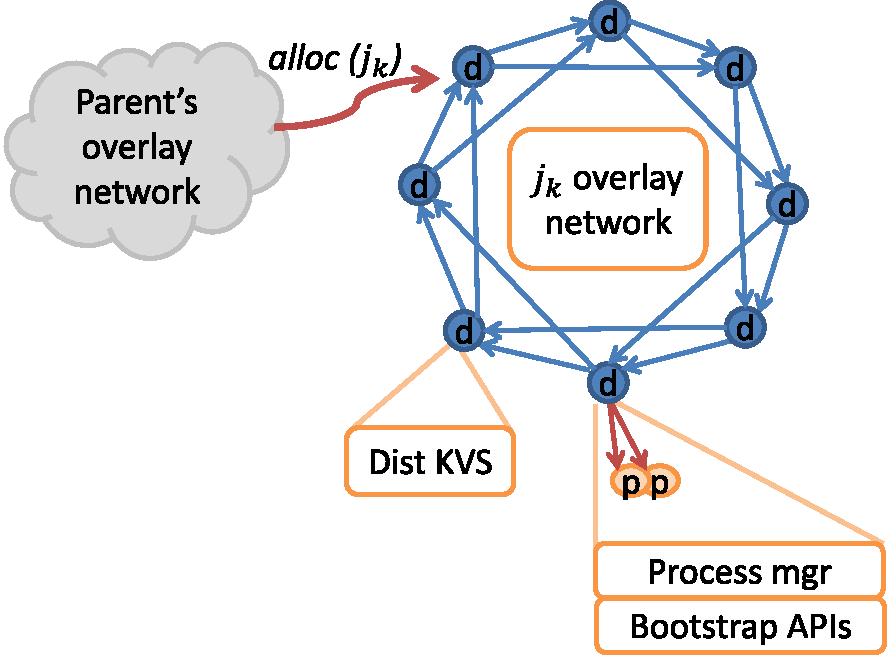
\includegraphics[width=3.0in]{WRAP_Base}
  \caption{Base WRAP architecture for $alloc(j_k, c_{j_k})$}
  \label{fig:base}
\end{figure}
In this section, we will walk through our WRAP software architecture 
and mechanisms that are needed to implement the proposed WRAP services.
We will first describe the base architecture that demonstrates
the basic WRAP capabilities of executing an LWJ on a set of compute
nodes, as our base resource type. 
Next, we will describe how we can extend this architecture
to enable other advanced services such abilities to synchronize 
two independent LWJs, to grow compute node resources allocated to an existing 
LWJ, and to handle other types of resources such as power.

\subsubsection{Base Architecture to Execute an LWJ}
Figure~\ref{fig:base} shows our base software architecture
that can provide a single LWJ ($j_k$) with WRAP service primitives:
$alloc()$,
$launch()$,
$bootstrap()$,
$contain()$,
$record()$, and
$query()$.
It assumes that the overlay network for $parent(j_k)$
already exists and that this existing network can support highly scalable,
resource-efficient communications for $j_k$ upon granting the $alloc(j_k)$ request. 
Our architeture requires that any overlay network instance recursively
supports communications of a child LWJ either
through an explicit instantiation of a separate overlay network
or through the existing overlay network. However, the latter model
requires to support a growth and/or reconfiguration
of the existing network to be elastic.\marginpar{\tiny Note that during the detailed 
design phase, WRAP and Comms Framework thrusts will co-design 
the actual communication mechanisms.}
WRAP then uses the overlay network for $j_k$ as well as
a key-value store to serve scalable process management
to $j_k$'s processes.
The following explains distributed key-value store mechanisms 
and key process management services in more detail.

\paragraph{Distributed Key-Value Store (DKVS)}
\label{sect:dkvs}
provides a scalable mechanism 
by which the processes of $j_k$ can
share arbitrary information in a key-value pair amongst them.
Conceptually, DKVS represents a global key-value tuple space
and any process of $j_k$ can store its data by associating them
with a unique key. To be memory-efficient,
however, DKVS must store the data in a distributed
manner. Thus, the overlay network of $j_k$ must be capable of hashing the key
to route its tuple to the home key-value store location. Global synchonization
mechanisms such as collective fense will be provided to force
memory consistency of DKVS across all processes.

Because our overlay network will have built-in routing
schemes to support requisite distribution schemes,
each home database itself can be a simple in-memory KVS.
It is for this reason that we we will first consider a readily available, simple
database implementation such as {\tt Redis}. 
Depending on our overlay network topology,
KVS can be fully distributed across all of the overlay network daemons.
An example topology to support the full distribution is a ``forest''
with $log(N)$ connections wherein any daemon can be
the root of a binomial tree.

Our DKVS will support a hierarchical tuple space for tighter
data encapsulation per LWJ, which can futher lead to a higher level of 
protection.
More specifically, when an LWJ is
allocated, a new name scope for that LWJ will be
created and information on the resource allocated
to that LWJ will be stored as part of the default $record$ service: e.g.,
$j_k$::resource $\rightarrow$ $<$ core\_count(1024), power\_bound(100kw), ... $>$.
This information is accessible by $j_k$ as well as
its immediate child LWJ $j_{k+1}$.
Similarly, when a daemon creates an MPI rank process, it will add the
personality of that process under this LWJ name scope
such as $j_k$::rank(128) $\rightarrow$ $<$ host IP, pid, executable path, ... $>$.
Finally, DKVS will allow any process of the LWJ to store arbitrary information
as part of $record(j_k, d_{j_k})$. All information stored
with $record$ will be pushed to $parent(j_k)$ when $j_k$
is destroyed. Thus, the information will ultimately find its place
in a persistent resource manager repository through the job hierarchy. In addition,
DKVS will further support $query$, providing the calling process
with underlying resource allocation infomation.

\paragraph{Scalable Process Management (ProcMan) Services}
\label{sect:procman}
can be implemented using the overlay network and DKVS as their 
basic scalable mechanisms. The scalable process management 
run-time services includes, but are not limited to, the following:

\begin{itemize}
\item{{\bf Bulk Process Creation and Stop}: The head daemon of the overlay network
receives a process creation request
through $launch(j_k, c_{j_k})$ and propagates that command to the rest of the daemons
in $O(log(N))$. Upon receiving the request, each daemon forks and execs
local processes. If the request contains an optional {\tt sync\_assist} flag, the daemons
stop the processes immediately after the creation to support a subsequent $sync()$ issued
by another LWJ. In either case, the daemons store
information on the created target processes such as their process id, executable path
and hostname, into the DKVS.}

\item{{\bf Scalable Propagation of Environments}: The head daemon receives the environment
variables list and propagates that to the rest of the deamons
in $O(log(N))$. The daemons then concatenate this master environment variables
list to their local environment variables and export them to their
processes. If the head daemon receives an optional $contain$ request, that
request is also being propagated. The specified containing-environment is used to contain
the target processes.}

\item{{\bf Process Mapping, Binding and Confinement}: The daemons provide the newly created processes
with topology information to support their mapping, binding and confinement to the underlying 
resources. The daemons retrieve the topology information from the key-value store.}

\item{{\bf Scalable {\tt stderr/stdout} Handling}: The daemons receive
{\tt stderr} and {\tt stdout}
from their processes and scalably push and merge them through a tree in the overlay
network towards the head daemon. Output aggregation techniques
will include ways to reduce the output progressively at every merge step
in the tree either by applying a readily available
reduction filter or a user-provided one.}

\item{{\bf Scalable signal/{\tt stdin} Forwarding}: The head daemon receives a UNIX signal
or an input through {\tt stdin} and scalably propagates it to a specified set of daemons
through a tree in the overlay network in $O(log(N))$. Upon receiving the signal or {\tt stdin},
each daemon routes it to their corresponding processes.}

\item{{\bf Scalable Process Termination Detection and Analysis}: When one or more processes
in the LWJ are normally or abnormally terminated, their home daemons detect the event and notify
the head daemon through a tree in the overlay network. A time-out filter can be used at every step of
the tree network to merge the return codes and, if abnormal, the stack traces of 
the terminated processes. Upon receiving the aggregated
event, the head daemon will clean up the entire LWJ and also present
to the users concise information about the termination.}

\end{itemize}


\paragraph{Unified Mechanism to Support Various Distributed Software Bootstrap Interfaces}
\label{sect:bootstrap}

DKVS will be designed to support a wide range of bootstrap interfaces
for distributed software including PMI 1 and 2~\cite{PMI2}, PMGR Collective and COBO,
LaunchMON~\cite{launchmon} and LIBI~\cite{libi}. With support for these interfaces
WRAP will be able to bootstrap a wide range of LWJs including a myriad of
MPI implementations, tools communication infrastructure such as MRNet
and also end-user tools such as STAT, TotalView and OpenSpeedShop.
Specifically, the PMI layers will be a very thin layer on top
of our DKVS implementation. We will support PMGR Collective,
COBO, LaunchMON, and LIBI such that each created process opens
up an ephemeral TCP port and store it as $j_k$::rank(128) $\rightarrow$ $<$ host IP, port $>$.
Then, each process in the binomial tree in these bootstrappers
will simply find the connection information of its parent as well as
its children using their ranks as the keys.

\subsubsection{Architectural Support for Job Function Synchronizations}
\label{sect:sync}
Our hierarchical job model has an ability to relate a job function
to another through $sync$.
For example, a tool may need to be co-located with an MPI job
and attached to its processes.
Thus, we must extend our base architecture to support that concept.
\begin{figure}
  \centering
    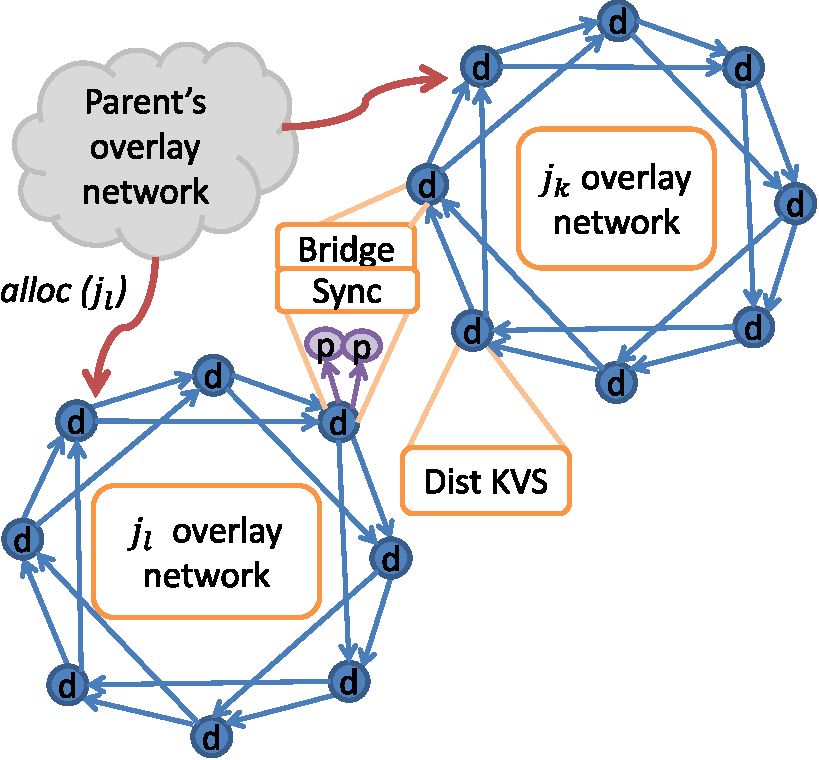
\includegraphics[width=3.0in]{WRAP_newJobFunction}
  \caption{WRAP architecture support for ${sync(j_k, j_l)}$}
  \label{syncext}
\end{figure}
As shown in Figure~\ref{syncext}, when $alloc(j_l)$
is granted for an additional new job function $j_l$,
the parent overlay network instantiates
another overlay nework for $j_l$ and helps manage
the processes of $j_l$ in the same manner as the base case.
To support ${sync(j_k, j_l)}$,
however, a connection needs to be made beween $j_l$'s
overlay and $j_k$'s overlay network.
For this purpose, we introduce the concept
of bridge. The bridge allows processes
of $j_l$ to be able to access DKVS of $j_k$, which includes
the mapping of the global MPI rank of a process of $j_k$
to its host name, pid, executable path~\cite{MPIRInterface},
information necessary for $j_l$ to locate all of $j_k$'s processes.
Alternatively, if the existing overlay network of $j_k$ is
capable of allocating and managing a new sibling job function
within itself, the need for a connection between two overlay
network and DKVS is eliminated.

\subsubsection{Architectural Support for Reallocation of Compute Nodes}
Our hierachical job model includes an ability to grow a job function $j_k$
by reallocating a new set of resources from the resources allocated
to $parent(j_k)$ and launching and bootstraping additional processes
across them.
Figure~\ref{fig:ext2} shows architectural support for that
job model.
\begin{figure}
  \centering
    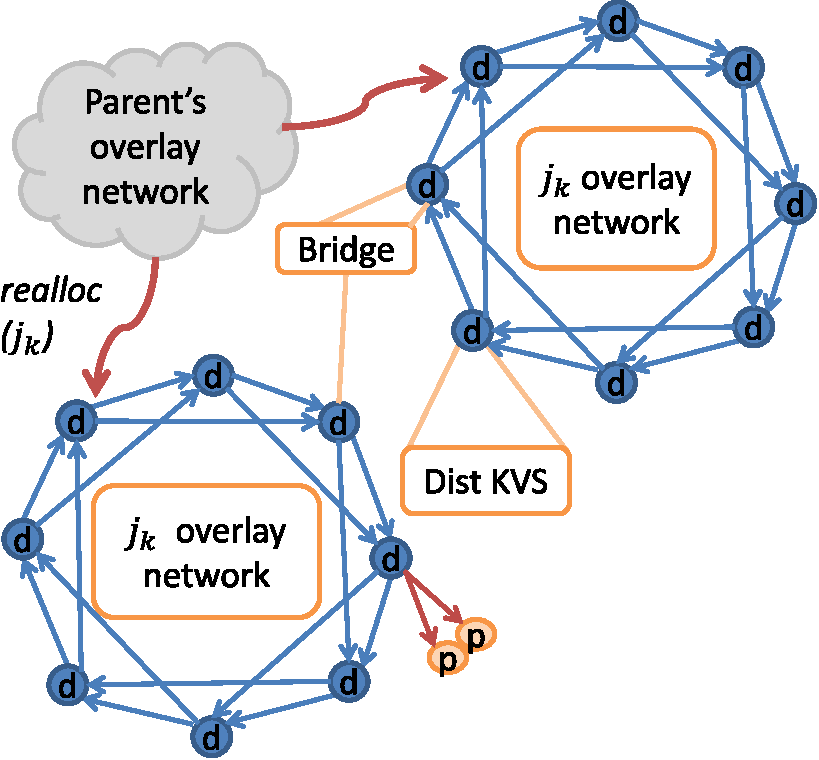
\includegraphics[width=3.0in]{WRAP_grow}
  \caption{WRAP architecture support for ${grow(j, cnew_j)}$}
  \label{fig:ext2}
\end{figure}
The scheme is essentially the same as that of $sync$.
Upon granting a reallocation of $rnew_j$,
$parent(j_k)$'s overlay network instantiates an overlay network
across $rnew_j$ and connects it to the existing overlay network
of $j_k$. The bridge support is again central for the connection.
Additional processes launched through the new network will
be able to access the DKVS associated with the existing $j_k$
name scope. Conversely, DKVS associated with these additional
processes will be made available to the existing $j_k$.
Alternatively, if the existing overlay network of $j_k$ is
capable of allocating and managing these additional processes
within itself, the need for a connection between two overlay
network and DKVS is eliminated. However, the existing overlay network
of $j_k$ is required to be capable of growing and
reconfiguring itself to cover the additional compute nodes.

\subsubsection{Architectural Support for Power as a Resource Type}
As $j$ will get the power bound allocated as a resource type,
a power control mechanism like RAPL~\cite{RountreeRAPL} can be used
to set the power bound of the allocated compute nodes.
The basic scheme computes the per-node power-bound average
and sets that averaged bound on each compute node.
For more advanced power-aware scheduling, groups of processes will
be assigned to new "power-domain" job functions using $split()$.
The new power-domain job functions will use $grow()$ and $shrink()$
operations described in Section~\ref{sect:hiop}
on the power bound as the resource type.
Although the distribution of power bound across compute
nodes will vary, our scheme will guarantee the aggregate power use
across all of these "power-domain" job functions bounded to the overall power bound
allocated to their parent.
These new job functions will create new name scopes
in the DKVS under their parent name scope:
e.g., $j_k$::$j_{k+1}$::resource $\rightarrow$ $<$ size(128), power\_bound(12.5kW) $>$.

\subsection{Component-Wise Work Breakdown}
In this section, we summarize the requirements and work items for
the major components of the proposed system.

\subsubsection{Overlay Network and Infrastructure Requirements}
The heart of WRAP lies in scalable and flexible overlay network support.
The overlay network's attributes that WRAP requires include:

\begin{itemize}

\item{an ability to support our elasticity model
efficiently and scalably through expanding and shrinking
compute nodes and job function processes launched on them;}

\item{an ability for an arbitrary head daemon to broadcast
or multicast data to a set of other daemons through a binomial
or binary tree with $O(log(number\_of\_daemons))$;}

\item{an ability for an arbitrary head daemon to aggregate data
sent from a set of other daemons through the binomial
or binary tree with $O(log(number\_of\_daemons))$;}

\item{an ability to allow both preset and custom-made reduction
opertators to reduce the aggregated data along the tree;}

\item{an ability to control data aggregation and reduction synchronously
with a mechanism to set an arbitrary time-out threshold: zero time-out means pass-through;
infinity time-out means global synchronization; and
in-between means partial synchronization with varying degrees;}

\item{an ability to route a key-value pair efficiently and
scalably by automatically hashing its key to find its home DKVS server
in support of get/put and global memory synchronization operations.}

\end{itemize}

\subsubsection{Process management}
To support scalable process management service described in Section~\ref{sect:procman},
the following components need to be investigated, designed and implemented:
\begin{itemize}
\item{an extensible communication protocol that allows
our process manager to conduct command and control
for all of its services;}
\item{a common data aggregation and reduction framework, techniques and API;}
\item{process management service components that
make use of the communication protocol and aggregation and reduction framework/API
and expose the services through high-level APIs;}
\item{executable commands such as a job function launcher that combines the
service components to implement certain types of process management
services for users;}
\item{topology-awared process binding and mapping components as well as
communication mapping APIs that client software can use for efficient
mappings between its communication patterns and the topology.}
\end{itemize}

\subsubsection{DKVS}
DKVS requires the following components:
\begin{itemize}
\item{name scoping specification and API;}
\item{direct get/put methods on a readily-available key-value server;}
\item{remote get/put methods on distributed key-value servers by
integrating servers to the communication infrastructure;}
\item{synchronization mechanisms and APIs that guarantee memory consistency
acorss the distributed servers.}
\end{itemize}

\subsubsection{Bootstrap Interfaces}
The following components should be implemented and demonstrated
using DKVS support:
\begin{itemize}
\item{PMI2 and port a version of MPICH as a reference implementation;}
\item{PMGR Collective and/or COBO and port a version of MVAPICH as a reference implementation;}
\item{LIBI and port a version of LIBI-enabled MRNet as a reference implementation.}
\end{itemize}

\subsubsection{Job Function Synchronization}
\begin{itemize}
\item{{\tt MPIR\_proctable} gatherer that gathers {\tt MPIR\_proctable} spread throughout the
DKVS into a centeral location including the address space of the job function launcher;}
\item{MPIR debug interface~\cite{MPIRInterface} that makes use of DKVS and process
management services to support parallel debuggers;}
\item{co-locator that co-locates an additional job function's processes with
the target processes;}
\item{LaunchMON Back-end API that makes use of DKVS to allow another job function processes
to discover the locations of target processes scalably.}
\end{itemize}

\subsubsection{Power Bound and Scheduling}
\begin{itemize}
\item{{\em split()} that allows an MPI job function to create smaller job functions, each with independent power bound control;}
\item{Dynamic power bound controller that manages expanding and shrinking of power bounds across these job functions.}
\end{itemize}

\subsection{Phase-Based Work Breakdown}
To bring up the proposed WRAP system progressively and expediently, we use a phased approach.
WRAP requires four phases: the outcome of earlier phases becomes the fundamental 
building blocks for the later phases.

\subsubsection{Phase 1: Basic Building Blocks (BBB) design}

\begin{table}
\centering
\begin{tabular}{|l|l|l|l|}
\hline
Work Item & Description & Dependency & Deliverable \\
\hline
\multirow{2}{*}{Protocol design} & design/prototype procMan & \multirow{2}{*}{comm. co-design} & \multirow{2}{*}{paper and review} \\
& command/control comm. protocol & & \\ \hline
\multirow{2}{*}{Aggregation/reduction design} & design/prototype aggregation &  \multirow{2}{*}{comm. co-design} & \multirow{2}{*}{paper and review} \\
& reduction framework and APIs & & \\ \hline
\multirow{2}{*}{DKVS name scoping design} & design/prototype name scoping & \multirow{2}{*}{comm. co-design} & \multirow{2}{*}{paper and review} \\
& specification and APIs & & \\ \hline
\multirow{3}{*}{Key-value store investigation}& evaluate key-value store servers & \multirow{3}{*}{none} & \multirow{3}{*}{finding summary} \\
& via direct put/get methods using & & \\
& bootstrap and MPIR emulation& & \\ \hline
\multirow{2}{*}{Power controller investigation} & investigate Intel RAPL &  \multirow{2}{*}{RM design} & \multirow{2}{*}{paper and review} \\
& and ways to control power bound & & \\ \hline
\end{tabular}
\caption{Phase 1 BBB design milestones and deliverables}
\label{tab:phase1}
\end{table}

During this phase, we will design and prototype the basic building blocks required
by WRAP. This layer represents the lowest building blocks for the WRAP thrust and has fundamental
dependecies on the overlay network infrastructure design as shown in Table~\ref{tab:phase1}.
Thus, they must be co-designed.

\subsubsection{Phase 2: Service Building Blocks (SBB) design and BBB implementation}
\begin{table}
\centering
\begin{tabular}{|l|l|l|l|}
\hline
Work Item & Description & Dependency & Deliverable \\
\hline
\multirow{2}{*}{ProcMan design} & design/prototype process manager & \multirow{2}{*}{comm. infra} & \multirow{2}{*}{paper and review} \\
& package and APIs & & \\ \hline
\multirow{2}{*}{Topo-aware binding design} & design/prototype topo-aware binding & \multirow{2}{*}{RM design} & \multirow{2}{*}{paper and review} \\
& and mapping mechanisms and APIs & & \\ \hline
\multirow{3}{*}{Remote DKVS} & investigate DKVS via & \multirow{3}{*}{comm. infra} & \multirow{3}{*}{finding summary} \\
& remote put/get/sync using bootstrap & & \\
& and MPIR emulation & & \\ \hline
\multirow{5}{*}{BBB Implementation} & implement ProcMan comm. protocol & \multirow{5}{*}{BBB proto} & \multirow{5}{*}{software drop} \\
& aggregation/reduction framework and API & & \\
& DKVS name scoping API & & \\
& direct key-value store & & \\
& power controller & & \\ \hline
\end{tabular}
\caption{Phase 2 SBB design milestones and deliverables}
\label{tab:phase2}
\end{table}

During this phase, we will use the design and prototypes of basic building blocks
to design and prototype higher-level service layer called service building blocks (SBB)
packages. In addition, that effort will further validate the BBB design and prototypes
and hence we will lock in the BBB design and produce production-quality BBB implementations
during this phase.
As shown in Table~\ref{tab:phase2}, this phase is designed to provide core WRAP functionality
engine except for the actual user interfaces to expose.

\subsubsection{Phase 3: User Service Interfaces (USI) design and SBB implementation}
\begin{table}
\centering
\begin{tabular}{|l|l|l|l|}
\hline
Work Item & Description & Dependency & Deliverable \\
\hline
\multirow{2}{*}{Job function utility design} & design/prototype job function utilities such & \multirow{2}{*}{SBB proto} & \multirow{2}{*}{paper and review} \\
& as job function launcher & & \\ \hline
\multirow{2}{*}{Job function sync design} & design/prototype job function & \multirow{2}{*}{SBB proto} & \multirow{2}{*}{paper and review} \\
& synchronizers & & \\ \hline
\multirow{2}{*}{PMI2, PMGR, LIBI design} & design/prototype boostrapers: & \multirow{2}{*}{SBB proto} & \multirow{2}{*}{finding summary} \\
& PMI2, PMGR/COBO and LIBI & & \\ \hline
\multirow{3}{*}{SBB implementation} & implement ProcMan package & \multirow{3}{*}{SBB proto} & \multirow{3}{*}{software drop} \\
& Topology-aware binding & & \\
& Remote DKVS & & \\ \hline
\end{tabular}
\caption{Phase 3 USI design milestones and deliverables}
\label{tab:phase3}
\end{table}

During this phase, we will use the design and prototype of service building blocks
to design and prototype the user-visible service layer called user service interfaces (USI).
In addition, once SBB prototypes are demonstrated that they are well-suited for the designed USI,
we will lock in the SBB design and produce production-quality SBB implementations.
As shown in Table~\ref{tab:phase3},
this phase will lay out the design of WRAP's external interfaces.

\subsubsection{Phase 4: USI implementation}
\begin{table}
\centering
\begin{tabular}{|l|l|l|l|}
\hline
Work Item & Description & Dependency & Deliverable \\
\hline
\multirow{2}{*}{Job function utility implementation} & implement job function& \multirow{2}{*}{NGRM framework} & \multirow{2}{*}{software drop} \\
& utilities such as launcher & & \\ \hline
\multirow{2}{*}{Job function sync implementation} & implement job function& \multirow{2}{*}{NGRM framework} & \multirow{2}{*}{software drop} \\
& job function synchronization & & \\ \hline
\multirow{2}{*}{PMI2, PMGR, LIBI design} & implement & \multirow{2}{*}{NGRM framework} & \multirow{2}{*}{software drop} \\
& PMI2, PMGR/COBO and LIBI & & \\ \hline
\end{tabular}
\caption{Phase 4 USI implementation}
\label{tab:phase4}
\end{table}

Once we demonstrate that USI prototypes sufficiently support both users and
other runtimes via reference implemenations, we lock in the SUI design and
produce production-quality USI implementations. Table~\ref{tab:phase4} shows
deliverables. The software drops will include the demonstration on client
software such as MPI, MRNet and other runtime tools.

\ifwbs
\newpage
\subsection{Workload Runtime WBS}

\begin{longtable}{|p{1cm}|p{10.2cm}|p{1cm}|p{1cm}|p{1.8cm}|}\hline
  \textbf{Item} & \textbf{Description}
                & \textbf{Deliv}\footnote{SD = software drop,
                        DR = design review, V = viewgraphs, D = document}
                & \textbf{Weeks} & \textbf{Depend} \\
  \hline
  \hline
  \multicolumn{5}{|l|}{4.1. \textbf{Runtime Basic Building Blocks}} \\
  \hline
  4.1.1.& Process manager command/control communication protocol design.
          (comms co-design)
        & DR, D
        & 
        & \\
  \hline
  \multicolumn{2}{|l|}{\em Note to Dong: agg/reduct framework moved to comms
              framework WBS}
        &
        &
        & \\
  \hline
  4.1.3.& Distributed key-value store name scoping specification and API.
          (comms co-design)
        & DR, D
        & 
        & \\
  \hline
  4.1.4.& Distributed key-value store investigation.  Evaluate servers
          via direct put/get methods using bootstrap and MPIR emulation.
        & V
        & 
        & \\
  \hline
  4.1.5.& Power control: Investigate  RAPL and ways to control power bound.
        & DR, D
        & 
        & RM \\
  \hline
  4.1.6.& Implement ProcMan communication protocol, DKVS name scoping API,
          direct key-value store, power controller.
        & SD
        & 
        & 4.1.1, 4.1.2, 4.1.3, 4.1.4, 4.1.5 \\
  \hline
  \multicolumn{5}{|l|}{4.2. \textbf{Runtime Service Building Blocks}} \\
  \hline
  4.2.1.& Process manager: design/prototype ProcMan and API.
        & DR, D
        & 
        & comms, 4.1.1\\
  \hline
  4.2.2.& Topo-aware binding: design/prototype binding and mapping
          mechanism and APIs.
        & DR, D
        & 
        & RM, 4.1.*\\
  \hline
  4.2.3.& Remote DKVS: investigate DKVS via remote put/get/sync using
	  bootstrap and MPIR emulation.
        & V
        & 
        & comms, 4.1.3(?), 4.1.4\\
  \hline
  4.2.4.& Implement ProcMan, topology-aware binding, remote DKVS.
        & SD 
        & 
        & 4.2.1, 4.2.2, 4.2.3 \\
  \hline
  \multicolumn{5}{|l|}{4.3. \textbf{Runtime User Service Interfaces}} \\
  \hline
  4.3.1.& Design/prototype job function utilities such as job function
          launcher.
        & DR, D
        & 
        & 4.2.1, 4.2.2, 4.2.3 \\
  \hline
  4.3.2.& Design/prototype job function synchronizers
        & DR, D
        & 
        & 4.2.1, 4.2.2, 4.2.3 \\
  \hline
  4.3.3.& Design/prototype bootstrappers: PMI2, PMGR/COBO, LIBI
        & V
        & 
        & 4.2.1, 4.2.2, 4.2.3 \\
  \hline
  4.3.4.& Implement job function utility.
        & SD
        & 
        & comms, 4.3.1 \\
  \hline
  4.3.5.& Implement job function sync.
        & SD
        & 
        & comms, 4.3.2 \\
  \hline
  4.3.6.& Implement PMI2, PMGR/COBO, LIBI
        & SD
        & 
        & comms, 4.3.3 \\
  \hline
\end{longtable}
\fi


\section{Project Schedule and Deliverables}
\label{sect:delivery}


\appendix
\section{Requirements}\label{Reqs}

\subsection{High Level Requirements}\label{ReqsHiLev}

\begin{tabular}{|p{4cm}|p{12cm}|}\hline
  \textbf{Scalable} & Resource Manager will scale up to 100,000 compute
	nodes per cluster and will scale to many clusters to allow
	management of even the largest centers \\
  \hline
  \textbf{Reliable} & Resource Manager will not have a single point of
	failure and shall never require scheduled downtime for software
	upgrades. Fault tolerance will be incorporated at every level. \\
  \hline
  \textbf{Secure} & Resource Manager will support wire protocols with
	built-in privacy and data integrity. \\
  \hline
  \textbf{Extensible} & Resource Manager will support plugins with clean
	interfaces wherever possible to facilitate collaboration,
	customization, and novel functionality. \\
  \hline
  \textbf{Research Friendly} & Resource Manager design will incorporate
	features that allow experimentation and research analysis,
	including the ability to export sanitized logs, job data, and
	the ability to run experimental features within the Resource
	Manager framework. \\
  \hline
  \textbf{Generalized} & Resource Manager will attain maximal flexibility
	by abstracting resources as much as possible. i.e., a compute node
	is a pool of resources, a cluster is a pool of resources, a center
	is a pool of resources, where a resource can be a consumable or a
	collection of such consumables. \\
  \hline
  \textbf{Integrated} & Resource Manager will allow easy integration with
	other tools and frameworks, including monitoring, logging, and
	remote execution. \\
  \hline
\end{tabular}

\subsection{Architectural Components}\label{ReqsArch}

\begin{tabular}{|p{4cm}|p{12cm}|}\hline
  \textbf{Scheduler} & The Scheduler manages the priorities of a queue
	of jobs requesting access to resources controlled by NGRM.\\
  \hline
  \textbf{Resource Manager} & Tracks resources available in the system and
	arbitrates access to these resources.\\
  \hline
  \textbf{Remote Execution} & Handles launch of processes across one or
	more resources managed by NGRM, including authorization,
	authentication and management of IO, environment, etc..\\
  \hline
  \textbf{Monitoring/Logging} & Manages collection and storage of monitoring
	and log data across the NGRM.\\
  \hline
  \textbf{Provisioning} & Manages root and other filesystem images across
	the NGRM.\\
  \hline
  \textbf{Communications Network} & Network channel through which all
	components of NGRM communicate.\\
  \hline
\end{tabular}

\subsection{High-Level Functional Requirements}\label{ReqsHiLevFun}

\begin{longtable}{|p{1cm}|p{15cm}|}\hline
  \multicolumn{2}{|l|}{1. \textbf{Zero Downtime}} \\
  \hline
  1.1. & Scheduled upgrades of NGRM components shall not require a downtime.\\
  \hline
  1.2. & The NGRM shall incorporate fault tolerance at every level, so
	that a failure of one component does not affect functionality of the
	system as a whole.\\
  \hline
  1.3 & The NGRM shall support version interoperability, so that the
	deployed system as a whole is not required to be at the same level
	of software.\\
  \hline
  \multicolumn{2}{|l|}{2. \textbf{Efficient Center-Wide Resource Management}} \\
  \hline
  2.1 & The NGRM shall have the ability to function as a single instance
	managing all clusters within a network. \\
  \hline
  2.2 & The NGRM shall be able to efficiently display a global view of
	resources to users when running in the mode described in R2.1.\\
  \hline
  2.3 & The NGRM shall support the specification of generic resources such
	as GPUs, IO Bandwidth, Power, etc in addition to CPUs, Memory,
	and nodes. \\
  \hline
  2.4 & The NGRM shall allow the hierarchy of resources to be specified in
	configuration or during discovery. For example, the definition of
	a node should allow the topology of that node to be recorded in
	the NGRM configuration (i.e. which CPUs are in which sockets,
	NUMA placement of memory, etc.) Similarly, there shall be the
	ability to record/discover the topology of nodes within a cluster,
	location and bandwith to IO storage from those nodes, access to
	and number of licenses, etc. FIXME: This needs rewording\\
  \hline
  2.5 & The NGRM shall support allocation of "interactive" resources from
	the compute pool, allowing more intelligent and dynamic creation
	of "login" nodes\\
  \hline
  2.6 & The NGRM shall support resource "tags" (similar to existing features)
	that can be applied to any resource, and a method to allow users
	requesting resources to select from tags\\
  \hline
  \multicolumn{2}{|l|}{3. \textbf{Integrated Monitoring and Logging}} \\
  \hline
  3.0 & NGRM monitoring and logging shall be designed to reduce system noise
	as much as possible\\
  \hline
  3.1 & NGRM shall provide an integrated monitoring plugin API to allow
	system monitoring to be extended to handle future requirements.\\
  \hline
  3.2 & NGRM shall provide the ability for users to tune the level of
	monitoring on the nodes of their jobs, allowing users to decrease
	monitoring levels and/or intervals for noise-sensitive jobs, or
	increase levels if they so choose.\\
  \hline
  3.3 & NGRM system monitoring events on resources connected with a particular
	job (including file systems) shall be made available to users
	monitoring their job or in post-mortem reports or queries.\\
  \hline
  3.4 & NGRM job log data shall have a public interface usable by tools
	such as sqlog to avoid duplication of data.\\
  \hline
  3.5 & NGRM job log and system monitoring data shall be made available in
	sanitized form for use in job scheduling research, simulator testing
	of NGRM releases, etc.\\
  \hline
  3.6 & NGRM job log and system monitoring data shall be collected,
	annotated, and saved to facilitate failure analysis.\\
  \hline
  3.7 & NGRM shall provide a library that can be linked to user codes that
	will collect and store generic key/value pairs.  This would replace
	LLNL's tracker tool and LANL's reportjob tools.\\
  \hline
  \multicolumn{2}{|l|}{4. \textbf{Communication Network}} \\
  \hline
  4.1 & NGRM components shall exchange messages and route log and monitoring
	data through a heirarchical, fault tolerant network.\\
  \hline
  4.2 & NGRM network shall support messages, streaming data, and RPCs\\
  \hline
  4.3 & NGRM network shall support privacy, integrity, and authentication\\
  \hline
  4.4 & NGRM network shall export a API for use by tools and users to reuse
	established global and job-wide communication hierarchy.\\
  \hline
  \multicolumn{2}{|l|}{5. \textbf{Remote Execution}} \\
  \hline
  5.1 & NGRM shall provide a service for remote parallel execution across
	jobs for users as well as globally for administrators\\
  \hline
  5.2 & NGRM remote execution service shall have the ability to manage
	instantiation of private namespaces for jobs\\
  \hline
  5.3 & NGRM remote execution shall allow transport of all process environment
	attributes including environment variables, resource limits,
	namespace attributes, etc.\\
  \hline
  5.4 & NGRM shall have the ability to bootstrap specialized environments
	such as a copy of NGRM itself (recursive execution), or an instance
	of \slurm\ (for backwards compatibility), or other frameworks such as
	Hadoop.\\
  \hline
  5.5 & NGRM shall support launch of MPI jobs up to 100,000 nodes with an
	arbitrary number of tasks per node.\\
  \hline
  \multicolumn{2}{|l|}{6. \textbf{Provisioning}} \\
  \hline
  6.1 & NGRM shall separate user and system execution envioronments by
	running within a minimal "core" system root, and invoking all jobs
	within separate (possibly user-selected) root filesystem\\
  \hline
  6.2 & NGRM shall provide service to allow users to run jobs with
	filesystem configuration of their choosing using private namespaces.
	The filesystems will need to be mounted without setuid for security
	purposes.\\
  \hline
  \multicolumn{2}{|l|}{7. \textbf{User Interface}} \\
  \hline
  7.1 & The NGRM shall export a rich API from which to build user interfaces.
	Command line as well as web based interfaces should be feasible with
	this API.\\
  \hline
  7.2 & NGRM should support a centralized data store for management and
	analysis of system usage. The store should support highly concurrent
	and frequent accesses in as close to real time as possible without
	affecting job performance. A memory-based database supporting a
	pub/sub mechanism, such as Redis, would be ideal. (Jeff Long,
	Joel Martinez)\\
  \hline
  7.3 & NGRM should provide an HTTP based REST API. Ideally the API would
	support a variety of different data formants (JSON, XML, etc...).
	The API should be implemented with a single-sign-on solution or
	API key implementation to avoid the need for additional user
	authentication. (Jeff Long, Joel Martinez)\\
  \hline
  \multicolumn{2}{|l|}{8. \textbf{Scheduling}} \\
  \hline
  8.1 & The Scheduler in the NGRM shall operate as a plugin or separate
	process or other easily replaceable component.\\
  \hline
  8.2 & The Scheduler API shall have a clean interface such that the
	scheduler does not need to be upgraded/developed in lockstep with
	the NGRM core\\
  \hline
  8.3 & The Scheduler interface in the NGRM shall allow the scheduling
	implementation access to all resources information gathered by
	the RM, including topology, heirarchy, data locality, IO bandwidth,
	etc.\\
  \hline
  8.4 & When running in recursive mode (e.g. see 5.3), the user should be
	allowed to select from a list of alternate scheduler implementations
	or even provide their own.\\
  \hline
  8.5 & NGRM scheduler shall support high job throughput\\
  \hline
  8.6 & NGRM shall support overlapping resource partitions (queues)
 	NGRM scheduler shall support complex job dependencies\\
  \hline
\end{longtable}

\subsection{Use Cases}\label{ReqsUseCases}

\begin{longtable}{|p{1cm}|p{15cm}|}\hline
  UC1 & \textbf{Use NGRM recursive execution to manage dedicated application
	test time}\newline
	Currently a DAT (dedicated application test) is managed
	by draining an entire cluster and then "giving" the test team access
	to the cluster via support staff with expedite privileges. With
	NGRM recursive execution, the DAT could be submitted to the RM as
	a job with constraints to run on all or part of a cluster. Once the
	job has been allocated on the cluster, team members would instantiate
	interactive instances to the job, and the recursive feature of NGRM
	would make it appear as if they had access to an empty cluster. Jobs
	could then be submitted to this instance from within the original
	NGRM job or the users' interactive instances. This scenario is also
	useful for testing new versions of the NGRM or other system software.\\
  \hline
  UC2 & \textbf{Sysadmin ability to "drain" only a portion of the resource
	hierarchy}\newline
	Currently, the resource management "drain" functionality is limited
	to a single node. Consider a case where a resource within a node goes
	bad, e.g. a GPU. Since the rest of the node is fine, the NGRM should
	allow just the GPU resource to be "drained" and the rest of the
	node is usable for compute jobs that do not need a GPU resource.
	When draining a full node or group of nodes, all the resources within
	the hierarchy of those nodes should also be drained. This would also
	allow an entire cluster or subset of resources to be drained by
	draining at the top level "cluster" resource.\\
  \hline
  UC3 & \textbf{Power utilization as a resource}\newline
	As a datacenter manager I want to deploy a cluster and provision less
	power to it than the max theoretical peak. The NGRM should allow the
	total available power to be specified at the cluster and/or PDU level
	within the cluster, and should treat power as a consumable resource.
	The NGRM will ensure that the set of resources use only the power that
	has been budgeted. If realtime power utilization is available, then
	those values can be aggregated and used (though this may not be safe
	when applications with fluctuating power demands are running),
	otherwise the NGRM should allow some kind of power utilization model
	to be registered (e.g. 90W per cpu + 100W per GPU + 200W base
	utilization per node...)\\
  \hline
  UC3.1	& \textbf{Energy usage part of job report}\newline
	The total energy consumed by a job should be reported upon job
	completion. (Barry Rountree)\\
  \hline
  UC3.2	& \textbf{Track power efficiency of components}\newline
	CPU's have varying power efficiency. Periodically measure this and
	record in resource db to be combined with a static power model.
	Also, scheduler could use this info to schedule the fastest nodes
	to the critical path. (Barry Rountree)\\
  \hline
  UC3.3	& \textbf{MPI runtime able to set power MSRs}\newline
	The MPI runtime can identify slow ranks and adjust power clamping
	to gain more performance. Application-driven variation in power
	consumption must not exceed breaker trip levels in a system plumbed
	for less than peak power consumption. (Barry Rountree)\\
  \hline
  UC3.4	& \textbf{Provide ability for job to specify power ranges}\newline
	User should be able to specify the maximum (and minimum?) power their
	job will consume.  Scheduler will only schedule job when it can
	configure the resources to remain within the specified power envelope.
	(Barry Rountree)\\
  \hline
  UC3.5	& \textbf{Node vs. Time Scheduling becomes Power vs. Time}\newline
	See M. Etinski paper~\cite{PowerOpt} (Barry Rountree)\\
  \hline
  UC4 & \textbf{Generic aggregate resources}\newline
	As a generic case of UC3, imagine a resource that is distributed
	across nodes or a whole cluster. A contrived example might be
	bandwidth to a SAN or other storage pool. The NGRM should have the
	ability to account for, manage, and schedule such generic resources
	in a way that is extensible to unforeseen resources, since we cannot
	imagine all possibilities beforehand. The NGRM should offer the
	ability to develop plugins or helpers to enforce and monitor and
	display these aggregate resources.\\
  \hline
  UC5 & \textbf{Center-wide cron}\newline
	As a sysadmin I may want to schedule a periodic job to run on
	systems of a certain type, so the NGRM should have cron-style
	capabilities at the center level. A cron "job" should be registered
	in the queue or in configuration that is run by the NGRM on the
	specified interval, on nodes matching the resource constraints
	specified in the "job". Cron work scheduled on compute nodes, such
	as required NAPS tests, should be run through NGRM such that they
	do not create OS jitter for running jobs. For example, they could
	only run between jobs or if they must run during a job, they could
	run synchronized. Users should be able to submit cron jobs too (at
	least some users like hotline do this).\\
  \hline
  UC6 & \textbf{Live user feedback for job progress}\newline
	As a user I would like access to resource manager data live while my
	job is running as a sort of job progress indicator. It would be useful
	to have IO statistics (perhaps with built-in IO Watchdog
	functionality), power utilization, network bandwidth, and the ability
	to register handlers if no progress is detected (by my own definition
	of no progress detected).\\
  \hline
  UC7 & \textbf{Allow users to inject application specific data into
	data stream for jobs}\newline
	As a user it would be really useful if I could inject application
	specific data into the data stream for a job. The job database could
	then keep this data in perpetuity, instead of having me keep data
	about my runs in an ad-hoc fashion. Data should be free form to allow
	for the greatest usability. Examples might be name of code, run ID,
	and iterations as they occur with timestamps. This would be useful in
	conjunction with UC6 as well.\\
  \hline
  UC8 & \textbf{dsh|dshbak}\newline
	As suggested by req. 5.1, pdsh|dshbak would be submitted via NGRM.
	There should be a way to limit concurrency (like pdsh fanout), a way
	to select specific hostnames (like pdsh wcoll), and a way to submit
	the dshback such that output is reduced in a distributed fashion
	(e.g. on intermediate nodes of the comms tree).\\
  \hline
  UC9 & \textbf{User control over system software levels}\newline
	As a user, for testing or reproducible results, I want to the ability
	to rerun a job or set of new jobs under a previously supported level
	of system software. I do not want to be required to record important
	system software versions manually, so the resource manager should
	track this data for every run and keep a record in a historical
	database so that I can go back and determine what software level
	was running when any one of my jobs ran.\\
  \hline
  UC10 & \textbf{Testing system software releases}\newline
	Major system sofware releases (e.g. TOSS major releases that break
	binary compatibility with old releases) should be testable in advance
	of being configured as the default through NGRM option at run time.\\
  \hline
  UC11 & \textbf{Integrated tool support}\newline
	NGRM should be able to efficiently launch and tear down STAT,
	totalview, and other distributed tools with a presence on compute
	nodes. NGRM should provide hooks for those tools so they can avoid
	reimplementing NGRM features. (See also MPI 3.0 Tools Support WG de
	Supinski, Schulz)\\
  \hline
  UC12 & \textbf{Allocate spare resources from a common pool}\newline
	Support a "spare resources" model whereby fault tolerant MPI jobs
	could dynamically pull in replacement nodes or other resources from
	the common pool rather than allocating spare resources privately at
	job submission.\\
  \hline
  UC13 & \textbf{Checkpoint/restart}\newline
	Support user-level checkpoint/restart such that NGRM can signal a
	job to begin checkpointing, receive an acknowledgement when
	checkpointing is complete, manage the checkpoint data (ensure it is
	on stable storage), clear the job from the system, then at a later
	time, stage in the checkpoint data and restart the job. (See also
	BLCR, SCR, OpenMPI c/r).\\
  \hline
  UC14 & \textbf{Ephemeral file system instances}\newline
	Allow user to request a dedicated parallel file system to be
	instantiated for the life of their job. NGRM could allocate disks
	from pool of storage resources, optionally stage data on/off of this
	file system at setup/tear-down.\\
  \hline
  UC15 & \textbf{Integrated I/O forwarding support}\newline
	Set up and tear down I/O forwarding daemons for exclusive use by
	a job. Allow flexibility in the number and placement of such daemons
	and their mapping to compute nodes. Collect I/O statistics from
	daemons and make available as part of job monitoring stream/records.\\
  \hline
  UC16 & \textbf{Hadoop framework}\newline
	NGRM should be able to launch hadoop framework on allocated resources
	(including storage).\\
  \hline
  UC17 & \textbf{User database instances}\newline
	NGRM should support starting a database server such as MySQL on
	allocated nodes/storage, loading a data set, and running a series of
	jobs that use the database, in some way telling the jobs how to
	connect to the server, and managing access.\\
  \hline
  UC18 & \textbf{Detect and report out of spec components}\newline
	As suggested by req. 3.6, NGRM should make it easy to detect when
	hardware / software components are performing out of spec or isolate
	components common to failed jobs.\\
  \hline
  UC19 & \textbf{Record HW configuration}\newline
	NGRM should record known HW configurations for each job executed.
	The data should have an schema-less, self-describing format to
	facilitate future previously unknown hardware configurations.\\
  \hline
  UC20 & \textbf{Provide "pre-job" resource information}\newline
	Users or admins should be able to query resource information such as
	network topology, I/O bandwidth, CPU speed, node memory, etc.
	This allows for users to alter jobs for "optimum" execution.
	For example, MPI communications algorithms or requested node
	allocation could be changed based on network topology.\\
  \hline
  UC21 & \textbf{Virtual private networks for jobs}\newline
	It should be possible to run a job in a virtual private network
	environment separate from that of the NGRM software, such that the
	job's network access is restricted to resources appropriate for it
	to access. This could be used to manage access to private services,
	such as the database in UC17. It might also be possible to organize
	user communities and their file stores such that the same protection
	offered by a firewall could be achieved without partitioning stateless
	compute resources.\\
  \hline
  UC22 & \textbf{Verbose Logging Triggered by Fault Event}\newline
	The monitoring system should facilitate capturing verbose debug logs
	prior to a fault event. One way to do this is with a circular trace
	buffer that is dumped into the monitoring stream on notification of
	a fault. (See "self propelled instrumentation", e.g. paradyn project)
	(Kathryn Mohror, Don Lipari)\\
  \hline
  UC23 & \textbf{I/O Staging}\newline
	The user should be able to specify files at job submission time that
	will be moved to storage close to compute nodes in advance of job
	launch. Files could be directed to be moved the other direction
	after job termination. This should be done in a way that does not
	impact other jobs, and can occur concurrently with allocating/freeing
	other job resources that aren't involved in moving files (Kathryn
	Mohror)\\
  \hline
  UC23 & \textbf{Give me a fat node for rank 0 and top it up with thin or fat ones}\newline
	In sbatch to ask for a fat node (more memory) and then a couple of
	other nodes (fat or thin), and then have the batch script start on
	the fat node, so that rank 0 is placed there by default by the MPI.
	(Kent Engstrom request to slurm-dev)\\
  \hline
\end{longtable}


\bibliographystyle{abbrv}
\bibliography{../bib/project,../bib/rfc}

\end{document}
